\documentclass[11pt]{article}
\usepackage[margin=1.05in]{geometry}
\usepackage{amsmath,amssymb,amsthm,mathtools}
\usepackage{booktabs,microtype,xcolor,graphicx}
\usepackage[shortlabels]{enumitem}
\usepackage[colorlinks=true,linkcolor=blue!45!black,citecolor=blue!45!black,urlcolor=blue!45!black]{hyperref}
\hypersetup{pdftitle={Vertex crossings in a symmetric Markov multinomial model},pdfauthor={Arjun Pemmasani}}
\newtheorem{theorem}{Theorem}[section]
\newtheorem{lemma}[theorem]{Lemma}
\newtheorem{proposition}[theorem]{Proposition}
\newtheorem{corollary}[theorem]{Corollary}
\theoremstyle{definition}
\newtheorem{definition}[theorem]{Definition}
\newtheorem{example}[theorem]{Example}
\theoremstyle{remark}
\newtheorem{remark}[theorem]{Remark}
\newcommand{\Z}{\mathbb Z}
\newcommand{\E}{\mathbb E}
\newcommand{\Prob}{\mathbb P}
\newcommand{\Var}{\operatorname{Var}}
\newcommand{\Cov}{\operatorname{Cov}}
\newcommand{\supp}{\operatorname{supp}}
\newcommand{\tree}{\operatorname{tree}}
\title{Vertex crossings in a symmetric Markov multinomial model}
\author{Arjun Pemmasani\\[2pt]
 \small Department of Mathematics, Harvey Mudd College\\
 \small Claremont, CA 91711, USA\\
 \small \texttt{apemmasani@hmc.edu}}
\date{}
\begin{document}
\maketitle

\begin{abstract}
We observe a ball bouncing down a Galton board with any number of directions. At each peg
it either keeps its direction with some fixed probability or randomly turns to one of
the other directions. Its bin measures how often it went each way, a
point of a simplex. When the ball rarely turns, the most likely bins are the
corners, which only a ball that never turns can reach. We ask when the best bin
of each face of the simplex becomes as likely as a corner. To first order every
face catches up at the same moment. We break this tie at second order, with an
explicit constant for each face. Hence on a long board, as the expected number of
turns grows to any fixed multiple of the length's logarithm, the most
likely bin jumps once, from the corners straight to the center. A nonuniform start or a weak external field changes the constants, potentially allowing an
intermediate face to win.
\end{abstract}

\medskip
\noindent\textbf{Keywords:} Potts chain; persistent random walk; Markov
multinomial distribution; occupation counts; mode; spanning trees.

\noindent\textbf{MSC2020:} 60J10; 60F05; 60F10; 82B20; 05C05; 33C10.

\section{Introduction}\label{sec:intro}

\subsection{The question and the answer}\label{sec:question}

Problem 131 of Kagey's Open Problem Collection~\cite{kagey131} is about a
Galton board on which the ball tends to keep going the same way. At the first
peg the ball goes left or right with probability $\frac12$, and at every later
peg it repeats its previous direction with probability $p$. Kagey asks when the
middle bin is exactly as likely as the two end bins. Our companion
paper~\cite{paperA}, Paper~A below, answers this for the persistent random walk,
or Ising chain with free ends. It compares each bin with an explicit Bessel
function, with an error bound that holds for every number of steps, and so traps
the tie in an explicit interval for every board. Kagey also asks what changes on
a tetrahedron. A natural version of that board sends the ball in one of three
directions at each peg, and the bins after $N$ steps form a triangle, one layer
of the tetrahedron.

Here we let the ball have $d\ge2$ directions. Its first direction is uniform,
and at each later peg it keeps going the same way with probability $p$
(otherwise it turns to one of the other $d-1$ directions, each with
probability $r=(1-p)/(d-1)$). After $N$ steps its bin is the vector
$n=(n_1,\ldots,n_d)$ of the numbers of steps in each direction. So the bins are
the points of a simplex, a segment for $d=2$ and a triangle for $d=3$. Only a
ball that never turns reaches a corner $Ne_i$, or vertex, so each vertex has
probability $p^{N-1}/d$.

When $p$ is close to $1$ the ball rarely turns, and the vertices are the most
likely bins. As $p$ decreases the other bins catch up. On the triangle there
are two natural candidates to catch up first, the middle of an edge, where the
ball has used two directions, and the middle of the triangle, where it has used
all three. We ask which one wins, and when.

Put $L=\log N$ and $T=Nr$. To first order every face of the simplex catches up
with the vertices at the same place, namely when $T$ is about $L$. So the first
order cannot answer the question. We break this tie at second order, and the
center of the whole simplex wins. For large $N$, as $T$ grows from $0$ to any
fixed multiple of $L$, the most likely bin jumps once, from the vertices
straight to the center, and no edge or other proper face holds it in between. On
the triangle the middle bin $(\frac N3,\frac N3,\frac N3)$ overtakes the corners
while the middles of the edges are still about $17\%$ below them.
Figure~\ref{fig:simplex} shows this at $N=24$.

\paragraph{Why every face ties.}
Take a face with $k$ directions. A ball that uses only these directions must
avoid the other $d-k$ directions at every peg, and it does so with probability
$(1-(d-k)r)^{N-1}\approx e^{-(d-k)T}$. So the face carries mass about
$\frac kde^{-(d-k)T}$, while a vertex carries $\frac1de^{-(d-1)T}$. On the face
the ball turns about $T$ times toward each direction, so the fractions $n_i/N$
fluctuate by about $1/\sqrt T$ around $1/k$. So the mass of the face is
spread over about $(N/\sqrt T)^{k-1}$ bins near its center, and
\[
\frac{\text{central bin of the face}}{\text{vertex}}
\approx\text{const}\cdot\Bigl(\frac{e^T\sqrt T}N\Bigr)^{k-1}.
\]
The bracket is the same for every face, and it crosses $1$ when
$T+\frac12\log T=L+O(1)$. Only the constant in front can tell the faces apart.

\paragraph{How second order breaks the tie.}
The constant is $e^{-(k-1)a_k}=k\det(2\pi\Sigma_k)^{-1/2}$, the mass $k$ of the
face over the Gaussian volume of the fluctuations, whose covariance is
$\Sigma_k/T$ (Proposition~\ref{prop:mass-balance}). So the ratio is
$\exp((k-1)[\Psi-a_k])$ with the common bracket $\Psi=T-L+\frac12\log T$, which
increases as $p$ decreases. Since $a_2>a_3>\cdots>a_d$, the full face reaches
the vertices first, when $\Psi=a_d$, while a face with $k<d$ directions is still
below them by the factor $e^{-(k-1)(a_k-a_d)}$. On the triangle this factor is
$e^{-(a_2-a_3)}=0.827$. After that moment the full center beats every proper
face, since $(d-1)(\Psi-a_d)>(k-1)(\Psi-a_k)$ when $\Psi\ge a_d$.

\subsection{Setting and notation}\label{sec:setting}

Fix $d\ge2$ and a start law $\mu$ on the set $[d]=\{1,\ldots,d\}$ of
directions, which we also call states. Let $X_1,X_2,\ldots$ be the Markov chain
with $X_1\sim\mu$ that keeps its state with probability $p\in[0,1]$ and moves to
each of the other $d-1$ states with probability $r=(1-p)/(d-1)$. Put
$\sigma=p-r=(dp-1)/(d-1)$. Kagey's board is $d=2$ with the uniform start.

\emph{Bins.} The count vector $K_N=(K_{N,1},\ldots,K_{N,d})$ records how often
each state occurs among $X_1,\ldots,X_N$. A bin is a vector $n$ of nonnegative
integers with sum $N$, and $P^\mu_N(n)=\Prob(K_N=n)$. For the uniform start
$\mu_i=1/d$ we write $P_N(n)$. The uniform start is the default everywhere
except in Section~\ref{sec:general-start}.

\emph{Faces and vertices.} A face is a nonempty set $F\subseteq[d]$, and
$\mu(F)=\sum_{a\in F}\mu_a$. A bin $n$ lies on the face
$\supp n=\{i:n_i>0\}$. The vertices are the faces of size $1$, that is, the
bins $Ne_i$. A word that reaches $Ne_i$ never switches, so
$P^\mu_N(Ne_i)=\mu_ip^{N-1}$, and for the uniform start we write
$V_N=p^{N-1}/d$.

\emph{Balanced bins.} A bin with $k$ positive coordinates is balanced if these
coordinates differ by at most $1$. For the uniform start all balanced bins with
$k$ positive coordinates have the same probability, since they differ only by a
permutation of the states. We call it $C_{N,k}(p)$, so $C_{N,1}=V_N$.

\emph{Scales.} Put $L=\log N$ and $T=Nr$. The expected number of switches (turns) is
$(N-1)(1-p)=(d-1)T(1-1/N)$, so $T$ is about the expected number of switches to
each other state. Put $\tau=T/L$. For $p>0$ let $u=r/p$, the odds of a switch
to one given state against no switch, and $z=Nu=T/p$. For $p>1/d$ we have
$\sigma>0$ and also use $v=r/\sigma=u/(1-u)$. Since $z-T=(d-1)Tz/N$, the scales
$z$ and $T$ differ by $O(L^2/N)$ when $T=O(L)$. This is smaller than every error
term in our asymptotic statements, so these statements hold with either one.
Exact statements are written in $u$.

\emph{Crossings.} For $2\le k\le d$, the crossing $p_{N,k}$ is the value of $p$
at which $C_{N,k}=V_N$, and $T_{N,k}=N(1-p_{N,k})/(d-1)$ is the value of $T$
there. We write $p^{(d)}_{N,k}$ when the number of states matters.

\emph{The constants.} For $k\ge2$ put
\begin{equation}\label{eq:intro-ak}
a_k=\frac12\log(4\pi)-\frac{k+\frac12}{k-1}\log k,\qquad
D_k=e^{-(k-1)a_k}=\frac{k^{k+1/2}}{(4\pi)^{(k-1)/2}},\qquad
\Psi_N(T)=T-L+\frac12\log T .
\end{equation}
Numerically $a_2=-0.4674$, $a_3=-0.6571$ and $a_4=-0.8139$.

\emph{Matrix form.} The transition matrix is $I+(T/N)Q$ with $Q=J-dI$, where $J$
is the all-ones matrix, so $Q$ switches at rate $1$ to each other state. The
exit rate of a face $F$ with $k$ states is $\lambda_F=d-k$, the principal
Dirichlet eigenvalue of $-Q$ on $F$.

\emph{Potts chain.} With the uniform start and $0<p<1$, a word $x_1\cdots x_N$
has probability $\frac1dr^{N-1}(p/r)^{\#\{s<N:\,x_s=x_{s+1}\}}$. This is the
one-dimensional $d$-state Potts model with free boundaries. For $d=2$ it is
the Ising chain of Paper~A.

\emph{Asymptotic notation.} In each statement the constants in $O(\cdot)$, and
the threshold behind ``for large $N$'', depend only on the quantities declared
fixed in that statement (always including $d$ and $k$). Uniformity in the other
variables is stated each time.

\subsection{Main results}\label{sec:results}

Theorem~\ref{thm:simplex-window} makes the heuristic of
Section~\ref{sec:question} precise. Uniformly for $cL\le T\le CL$, the
logarithm of $C_{N,k}/V_N$ is $(k-1)[\Psi_N(T)-a_k]$, up to a next term
$-(k-1)/(8T)$ that is again proportional to $k-1$ and an error
$O(T^{-2}+T^2/N)$. Part~(ii) of that theorem is the first-order statement. With
$T=\tau L$, a balanced bin on a face $F$ has probability
$\exp(-L[\tau\lambda_F+|F|-1]+O(\log L))$. At $\tau=1$ the exponent
$\tau\lambda_F+|F|-1$ equals $d-1$ for every face, so the first order cannot
choose.

By Theorem~\ref{thm:simplex-crossing}, for every $N\ge k$ the balanced bin with
$k$ positive coordinates crosses the vertices at exactly one $p_{N,k}$, which
increases with $N$, and
\begin{equation}\label{eq:intro-crossing}
T_{N,k}+\frac12\log T_{N,k}=L+a_k+\frac1{8T_{N,k}}+O(L^{-2}).
\end{equation}
For $d=2$ the model is the persistent random walk of Paper~A. For $k=2$
equation~\eqref{eq:intro-crossing} is the crossing equation of Paper~A
\cite[Proposition~3.8]{paperA}, and $a_2=\frac12\log(\pi/8)$ is its constant
$c_0$. Since $a_2>a_3>\cdots>a_d$, Corollary~\ref{cor:simplex-modes} shows that
for large $N$ and all $T\le CL$ the global mode changes exactly once, from the
$d$ vertices straight to the balanced bins with $d$ positive coordinates. All the
face-center crossings lie in a $p$-interval of length $(d-1)(a_2-a_d+o(1))/N$.
For small $N$ this can fail. On the triangle with $N=4$ an edge center can be
the mode (Example~\ref{ex:simplex-edge-mode}).

The same method gives the crossing of every bin whose positive coordinates are
of order $N$ (Theorem~\ref{thm:simplex-interior}). For fractions $\alpha$ its
constant is $D(\alpha)=A^2/\sqrt{\det(2\pi\Sigma_\alpha)}$ with
$A=\sum_i\sqrt{\alpha_i}$, where $\Sigma_\alpha$ is the occupation covariance of
a tilted chain, and $\det\Sigma_\alpha$ is a weighted count of the spanning
trees of the complete graph $K_k$ (Proposition~\ref{prop:kirchhoff}). At the
center the count is Cayley's $k^{k-2}$, and $D(\alpha)=D_k$.

Then we perturb the model in two ways. Each acts at order $1$, namely the
order of the constants $a_k$. A start law $\mu$ changes the constant of a face
$F$ against a vertex $i$ to $a_k+\frac1{k-1}\log(k\mu_i/\mu(F))$
(Theorem~\ref{thm:start-crossings}). The best bin of each face keeps the share
$\mu(F)/k$ of the uniform value (Theorem~\ref{thm:start-maxima}), so each face
gets a line in $t$ and the highest line holds the mode
(Corollary~\ref{cor:start-modes}). On the triangle with
$\mu=(\frac12,\frac12,0)$ this lets an edge hold the mode on a window of width
$\log(16/(9\sqrt3))=0.026$ in $T$ (Example~\ref{ex:K3-start}). A Potts field of
size $h_i/N$ per visit to state $i$ adds to each face the field averaged over
the face (Theorem~\ref{thm:weakfield-phases}), and one field makes every support
size win in turn (Corollary~\ref{cor:weakfield-full-hierarchy}).

Finally we drop the assumption that the positive coordinates are of order $N$.
A Bessel majorant has relative error $O(L^2/N)$ for every positive count vector
when $T=O(L)$ (Theorem~\ref{thm:uniform-simplex-majorant}). When at least two
coordinates are of order $N$, a small coordinate starts to matter once it has
size $N/L^2$ (Theorem~\ref{thm:simplex-boundary-crossover}). Near a vertex,
with one large count $b$ and small counts of total $o(b)$, the crossing odds
are $u=\sqrt{y/b}\,(1+o(1))$, where $y$ is the root of a product of Laguerre
polynomials (Theorem~\ref{thm:vertex-uniform-root}).

Section~\ref{sec:verify} describes the checks and lists open questions, and
the longer proofs are in Appendices~\ref{app:thresholds}
to~\ref{app:vertex}.

\subsection{Related work}\label{sec:related}

The law belongs to the theory of Markov multinomial distributions.
Edwards~\cite{edwards1960} introduced the Markov binomial distribution. Let
$\mu$ be a law on the two outcomes of a trial, success and failure. His trials
form a stationary chain with law $\mu$ at each trial that moves from $i$ to $j$
with probability $\theta\delta_{ij}+(1-\theta)\mu_j$. He wrote the generating
function of the number of successes as a product of matrices. Wang and
Yang~\cite{wangyang1995} extended this chain to finitely many states. We have
not seen their paper, and we describe it through Johnson, Kotz and
Balakrishnan~\cite[Chapter~35, Section~13.2]{jkb1997}. The chain of Wang and
Yang starts from a law $\mu$ and moves from $i$ to $j$ with probability
$\theta\delta_{ij}+(1-\theta)\mu_j$, where $0\le\theta\le1$, and the generating
function of its vector of category counts is a product of matrices. Our chain
with the uniform start and $p\ge1/d$ is the case where $\mu$ is uniform and
$\theta=\sigma$. So the exact law for the uniform start is a special case of
this theory, and we do not claim it as new. Our general start changes only the
initial law and keeps the uniform switching, so it is a Wang--Yang chain only
when $\mu$ is uniform. Hsiau~\cite[Theorem~1]{hsiau1997} proves compound
Poisson limits for sums over multistate chains with one nearly absorbing state,
and Wang and Tang~\cite{wangtang2003} prove Poisson-type limits for additive
processes on Markov chains. Whittle~\cite[formula~(8)]{whittle1955} gave the
exact law of the transition counts of a finite chain. The count vector is
determined by the transition counts and the first state, so $P_N$ could also be
summed from his formula.

Brydges, van der Hofstad and K\"onig~\cite{brydges2007} give occupation
densities for continuous-time chains on the visited faces of the simplex.
Huang, Kious, Sidoravicius and Tarr\'es~\cite[Theorem~1]{huang2018} give the
joint density of the local times, the last-exit spanning tree and the net
crossing numbers of a walk with symmetric conductances, with Bessel functions. Stadje~\cite[Theorems~1 and~2]{stadje1999} gives the generating
functions of the joint numbers of visits of a finite chain. He also proves limit
laws when one state becomes nearly absorbing and the chain leaves it with
probability of order $1/N$~\cite[Theorems~3 and~4]{stadje1999}. The other rows
of his transition matrix stay fixed, so the counts of the other states stay
bounded. Dietz and Sethuraman~\cite{dietz2007} study chains that switch from
$i$ to $j$ at time $n$ with probability $G(i,j)/n$. They make about $\log N$
switches by time $N$, but only $O(1)$ of them after time $N/2$, and their
occupation fractions have a limit law on the simplex. Our chain makes about
$(d-1)\log N$ switches near the crossings, spread evenly in time. Dupuis and Liu~\cite{dupuisliu2015} give the rate function of
the occupation measure, which we compare with our exponent in
Section~\ref{sec:simplex-thresholds}. Kassan-Ogly and
Filippov~\cite{kassanogly2003} solve the Potts chain in a field in the
thermodynamic limit. Their paper was not accessible to us through standard
means or institutional libraries, but its abstract and introduction are free
online, and we use nothing beyond these. Aside from this, no source we could
read compares one count vector with a vertex when $p$ depends on $N$, and none
of them finds the face-center crossings or the tie.
We take the Bessel and Laguerre formulas from~\cite{dlmf}.

\section{The model and the exact law}\label{sec:multistate-model}

We write $P^\mu_N$ in three forms. The \emph{run form} counts the switches,
and it gives all our exact statements. The \emph{refresh form} uses the
transition matrix $\sigma I+rJ$. When $p\ge1/d$ the chain keeps its state with
probability $\sigma$ and otherwise draws a fresh state uniformly from all $d$
states, possibly the same one. The \emph{ratio form} is the refresh form
divided by a vertex (so it measures a bin in units of a corner). For $p>1/d$ it is a sum of positive terms, and all our
asymptotics start from it.

For a positive count vector $n=(n_1,\ldots,n_k)$ with total $N$ and a state
$a$, let $W^{(a)}_n(j)$ be the number of words with counts $n$ and $j$ changes
that start with $a$, and let $W_n(j)=\sum_aW^{(a)}_n(j)$. Put
\[
S^{(a)}_n(u)=\sum_jW^{(a)}_n(j)u^j,\qquad
S_n(u)=\sum_aS^{(a)}_n(u)=\sum_jW_n(j)u^j .
\]
These polynomials do not depend on $d$. For a bin $n$ with some zero
coordinates, $S_n$ and $S^{(a)}_n$ mean the polynomials of its positive
coordinates.

\begin{proposition}[the generating function]\label{prop:dgf}
Put $y_i=x_it/(1-\sigma x_it)$ and $P^\mu_0(0,\ldots,0)=1$. As formal power
series,
\[
\sum_{N\ge0}\sum_{n_1+\cdots+n_d=N}P^\mu_N(n)\,x_1^{n_1}\cdots x_d^{n_d}\,t^N
=1+\frac{\sum_i\mu_iy_i}{1-r\sum_iy_i}.
\]
\end{proposition}

\begin{proof}
Let $F_i$ be the generating function of the words of length at least $1$ that
end in state $i$, each weighted by its probability, and let $S=\sum_iF_i$.
Conditioning on the last letter gives
$F_i=x_it\bigl(\mu_i+pF_i+r(S-F_i)\bigr)=x_it(\mu_i+\sigma F_i+rS)$, that is,
$F_i=y_i(\mu_i+rS)$. Summing over $i$ gives
$S=\sum_i\mu_iy_i+rS\sum_iy_i$, and the generating function is $1+S$.
\end{proof}

\begin{proposition}[the exact law]\label{prop:dpmf}
Let $N\ge1$, let $n$ be a bin, and put $F=\supp n$. Sums over $m$ run over the
integer vectors with $m_i=0$ for $i\notin F$ and $1\le m_i\le n_i$ for
$i\in F$, and $M=\sum_im_i$.
\begin{enumerate}[(a)]
\item (refresh form) With $0^0=1$,
\[
P^\mu_N(n)=\sum_m\Bigl(\sum_{i\in F}\mu_im_i\Bigr)\frac{(M-1)!}{\prod_im_i!}\,
r^{M-1}\sigma^{N-M}\prod_{i\in F}\binom{n_i-1}{m_i-1}.
\]
For the uniform start this reads
\[
P_N(n)=\frac1d\sum_m\frac{M!}{\prod_im_i!}\,
r^{M-1}\sigma^{N-M}\prod_{i\in F}\binom{n_i-1}{m_i-1}.
\]
\item (run form) If $p>0$, then $P^\mu_N(n)=p^{N-1}\sum_{a\in F}\mu_aS^{(a)}_n(u)$.
In particular $P_N(n)/V_N=S_n(u)$.
\item (ratio form) If $1/d<p<1$, so that $0<u<1$ and $v>0$, then
\begin{equation}\label{eq:simplex-positive-sum}
S_n(u)=(1-u)^{N-1}\sum_mM!\,v^{M-1}\prod_{i\in F}\frac1{m_i!}\binom{n_i-1}{m_i-1},
\end{equation}
which is a sum of positive terms.
\end{enumerate}
\end{proposition}

When $\sigma\ge0$, the refresh form has a direct reading. Cut the word into $M$
blocks at the $M-1$ refreshes. Each refresh lands on a prescribed state with
probability $r$, and each of the other $N-M$ steps keeps the state with
probability $\sigma$. If $m_i$ blocks carry state $i$, there are
$m_i(M-1)!/\prod_jm_j!$ orders of the block labels that start with $i$, and
$\binom{n_i-1}{m_i-1}$ ways to choose the lengths of the $m_i$ blocks of state
$i$. The proof below does not need $\sigma\ge0$.

\begin{proof}
(a) By the proof of Proposition~\ref{prop:dgf},
$S=\sum_{M\ge1}r^{M-1}\bigl(\sum_i\mu_iy_i\bigr)\bigl(\sum_iy_i\bigr)^{M-1}$. By the
multinomial theorem the coefficient of $\prod_iy_i^{m_i}$ in
$(\sum_i\mu_iy_i)(\sum_iy_i)^{M-1}$ is $\sum_i\mu_im_i(M-1)!/\prod_jm_j!$. With
$w_i=x_it$ we have $y_i=w_i/(1-\sigma w_i)$, and
$[w^j](w/(1-\sigma w))^m=\binom{j-1}{m-1}\sigma^{j-m}$ for $j\ge m\ge1$. For
$m=0$ only $j=0$ contributes. Multiplying the coefficients proves (a), and for
the uniform start $\sum_i\mu_im_i=M/d$.

(b) A word that starts with $a$ and has $j$ changes has probability
$\mu_ap^{N-1-j}r^j=\mu_ap^{N-1}u^j$. Sum over the words with counts $n$.

(c) Divide the uniform case of (a) by $V_N=p^{N-1}/d$. Since $r/p=u$ and
$\sigma/p=1-u$, we have
$r^{M-1}\sigma^{N-M}/p^{N-1}=u^{M-1}(1-u)^{N-M}=(1-u)^{N-1}v^{M-1}$.
\end{proof}

At $p=1/d$ we have $\sigma=0$ and only $M=N$ survives, which gives the
multinomial law for the uniform start. At $p=1$ only $M=1$ survives, which gives
mass $\mu_i$ at $Ne_i$. For $\sigma<0$ the terms in (a) can cancel, so for
numerical work we then use exact arithmetic or dynamic programming.

\subsection{Bessel bounds}

For $x\ge0$ the modified Bessel function of order $1$ is
$I_1(x)=\sum_{j\ge0}(x/2)^{2j+1}/(j!(j+1)!)$. Since
$\binom{2j+1}j\le4^j$, comparing coefficients gives $I_1(x)\le\sinh x\le e^x$.
We also use the expansion~\cite[Eqs.~10.40.1 and~10.17.1]{dlmf}
\[
I_1(x)=\frac{e^x}{\sqrt{2\pi x}}\Bigl(1-\frac3{8x}+O(x^{-2})\Bigr),
\qquad x\to\infty,
\]
and the function
\[
\Phi(x)=\sum_{j\ge0}\frac{x^j}{j!(j+1)!}=\frac{I_1(2\sqrt x)}{\sqrt x},
\qquad\Phi(0)=1 .
\]
Since $\binom{2j}j\le4^j$, we have $1/(j!(j+1)!)\le4^j/(2j)!$, and comparing term
by term with the even part of the series of $e^{2\sqrt x}$ gives
$\Phi(x)\le e^{2\sqrt x}$. Lemmas~\ref{lem:bessel-law}, \ref{lem:clipped-product}
and~\ref{lem:gaussian-phi-average} in Appendix~\ref{app:thresholds} give the
other facts about $\Phi$ that we use.

\section{The tie and its resolution}\label{sec:simplex-thresholds}

In this section the start is uniform. We prove the tie of
Section~\ref{sec:question} and break it (Subsection~\ref{sec:tie}), write the
constants as Gaussian volumes and spanning-tree sums
(Subsection~\ref{sec:gaussian-volumes}), and find the global mode
(Subsection~\ref{sec:global-mode}). The constants $a_k$, $D_k$ and $\Psi_N$ are
those of~\eqref{eq:intro-ak}. Let $n$ be a balanced vector with $k$ positive
coordinates and total $N$. By Proposition~\ref{prop:dpmf}(b),
$C_{N,k}/V_N=S_n(u)$, and as a function of $u$ this ratio does not depend
on $d$.

\subsection{Every face ties at first order}\label{sec:tie}

\begin{theorem}[every face ties at first order]\label{thm:simplex-window}
Fix $d\ge2$ and $0<c<C$.
\begin{enumerate}[(i)]
\item For large $N$, uniformly for $cL\le T\le CL$ and $2\le k\le d$,
\[
\log\frac{C_{N,k}}{V_N}=(k-1)\bigl[\Psi_N(T)-a_k\bigr]-\frac{k-1}{8T}
+O\Bigl(\frac1{T^2}+\frac{T^2}N\Bigr).
\]
\item Put $T=\tau L$. Uniformly for $c\le\tau\le C$ and $1\le k\le d$, a face
$F$ with $k$ states has
\[
\log C_{N,k}=-L\bigl[\tau\lambda_F+k-1\bigr]+O(\log L),\qquad\lambda_F=d-k .
\]
At $\tau=1$ the right side is $-(d-1)L+O(\log L)$ for every $k$.
\item Put $T=L-\frac12\log L+t$. Uniformly for $t$ in a compact interval, for
each $2\le k\le d$,
\begin{equation}\label{eq:simplex-window}
\frac{C_{N,k}}{V_N}\longrightarrow e^{(k-1)(t-a_k)} .
\end{equation}
\item $a_2>a_3>\cdots$.
\end{enumerate}
\end{theorem}

In words, the central bin of every face reaches the vertices when $\Psi_N(T)$
is of order $1$, that is, when $T=L-\frac12\log L+O(1)$. Part (ii) is the
first-order statement: on the scale $L$ all faces have the same exponent at
$\tau=1$. Part (iii) zooms into the window where the tie lives. There each ratio
has a limit, and the faces differ only through the constants $a_k$. Paper~C
describes such tie windows in general, and Remark~\ref{rem:sticky} explains why
among symmetric kernels only the uniform one ties on every face.

\begin{theorem}[face-center crossings]\label{thm:simplex-crossing}
For every $2\le k\le d$ and $N\ge k$ there is exactly one $p=p_{N,k}\in(0,1)$
with $C_{N,k}(p)=V_N(p)$. The balanced bin is more likely than a vertex below
$p_{N,k}$ and less likely above it. The crossing $p_{N,k}$ is strictly
increasing in $N$,
\[
p_{k,k}=\frac1{1+(d-1)(k!)^{-1/(k-1)}},
\]
and every crossing has $u\le(k!)^{-1/(k-1)}<1$, so $p_{N,k}>1/d$. For fixed $k$
the value $z_{N,k}=N(1-p_{N,k})/(d-1)$ of $T$ at the crossing satisfies
\[
z_{N,k}+\frac12\log z_{N,k}=L+a_k+\frac1{8z_{N,k}}+O(L^{-2}),
\]
and
\begin{equation}\label{eq:simplex-root-expansion}
z_{N,k}=L-\frac12\log L+a_k
+\frac{\frac14\log L-\frac12a_k+\frac18}{L}
+O\Bigl(\frac{(\log L)^2}{L^2}\Bigr).
\end{equation}
\end{theorem}

In words, each face center crosses the vertices exactly once, the crossing
moves towards $p=1$ as $N$ grows, and the crossing equation is the same for
every face except for the constant $a_k$. For $d=2$, $z_{N,2}=N(1-p_N)$ is the
crossing $z_N$ of~\cite{paperA}, and $a_2=\frac12\log(\pi/8)$ is its constant
$c_0$. The proofs here do not use the binary case.
Figure~\ref{fig:simplex} shows the full-center crossing on the triangle at
$N=24$.

\begin{figure}[t]
\centering
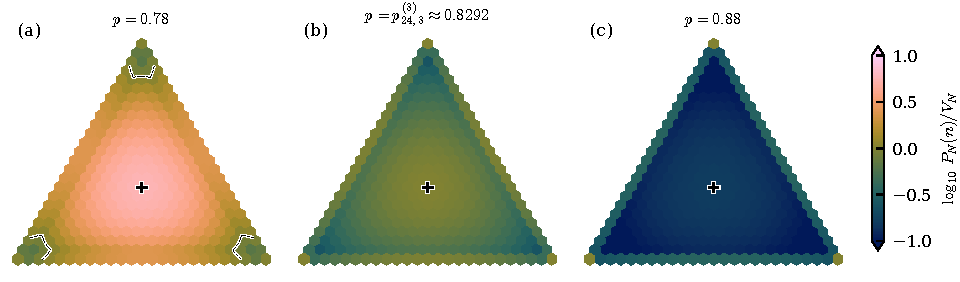
\includegraphics{figures/simplex}
\caption{The ratio $P_N(n)/V_N$ for $d=3$ and $N=24$, one hexagon per bin, on
a $\log_{10}$ scale. (a) At $p=0.78$ only the $21$ bins inside the dashed
curves near the vertices are below the vertex height. (b) At the full-center
crossing $p^{(3)}_{24,3}=0.82921\ldots$ the center $(8,8,8)$ (cross) ties with
the vertices and every other bin is below them. (c) At $p=0.88$ every
nonvertex bin is below the vertex height.}
\label{fig:simplex}
\end{figure}

\paragraph{Idea of the proofs.}
The proofs are in Appendix~\ref{app:thresholds}. The exact part uses the run
form. The polynomial $S_n$ has nonnegative coefficients, and its first nonzero
coefficient is $W_n(k-1)=k!$, from the words that use each state in a single
run. So $S_n$ increases from $0$ to $\infty$ and crosses $1$ exactly once. Its
next coefficient $W_n(k)=k!(k-1)(N-k)/2$ grows with $N$, which moves the root.
The asymptotic part uses the ratio form~\eqref{eq:simplex-positive-sum}. This
sum is close to a Bessel integral (Theorem~\ref{thm:uniform-simplex-majorant}),
and the Laplace expansion of this integral (Lemma~\ref{lem:no-rare}) gives, for a
balanced $n$ with $k$ positive coordinates and uniformly for
$cL\le z\le CL$,
\begin{equation}\label{eq:simplex-uniform-ratio}
S_n(z/N)=D_k\frac{z^{(k-1)/2}e^{(k-1)z}}{N^{k-1}}
\Bigl(1-\frac{k-1}{8z}+O\Bigl(\frac1{z^2}+\frac{z^2}N\Bigr)\Bigr).
\end{equation}
This is the heuristic of Section~\ref{sec:question} with all constants. Then
$\log V_N=-(d-1)T-\log d+O(T^2/N)$ and $z-T=O(L^2/N)$ give parts (i) to (iii)
and the expansions of the crossing. Part (iv) follows from the monotonicity of
$(x+\frac12)\log x/(x-1)$.

\subsection{The constants as Gaussian volumes}\label{sec:gaussian-volumes}

The heuristic of Section~\ref{sec:question} says that $D_k$ should be the mass
of a face divided by the Gaussian volume of the fluctuations of the fractions.
We now make this precise in 2 ways. First we find the crossing at every
interior point of a face and write its constant with a covariance matrix and a
spanning-tree sum (Proposition~\ref{prop:kirchhoff}). Then we sum over the whole
face (Proposition~\ref{prop:mass-balance}). We evaluate the constants at the
actual fractions $\alpha_i=n_i/N$, since we do not assume that the count vector
converges at any rate.

\begin{theorem}[interior compositions]\label{thm:simplex-interior}
Fix $k\ge2$, $\varepsilon>0$ and $0<c<C$. Let $n_1+\cdots+n_k=N$ with
$\alpha_i=n_i/N\ge\varepsilon$, and put
\[
A=\sum_{i=1}^k\sqrt{\alpha_i},\qquad g=A^2-1,\qquad s=k-1,\qquad
D(\alpha)=\frac{A^{k/2+1}(\prod_i\alpha_i)^{-3/4}}{(4\pi)^{s/2}}.
\]
Uniformly for these count vectors and $cL\le z\le CL$,
\begin{equation}\label{eq:simplex-interior-ratio}
S_n(z/N)=D(\alpha)\frac{z^{s/2}e^{gz}}{N^s}
\Bigl(1+O_{k,\varepsilon,c,C}\bigl(z^{-1}+z^2/N\bigr)\Bigr).
\end{equation}
The unique positive root $u_n$ of $S_n(u)=1$ satisfies
\begin{equation}\label{eq:simplex-interior-root}
Nu_n=\frac sgL-\frac s{2g}\log L
-\frac{\log D(\alpha)+(s/2)\log(s/g)}g
+O_{k,\varepsilon}\Bigl(\frac{\log L}L+\frac{L^2}N\Bigr).
\end{equation}
For a fixed target $\alpha$ and counts $n_i=N\alpha_i+O(1)$, the constants may be
evaluated at the target without changing the error order.
\end{theorem}

In words, a bin with fractions $\alpha$ grows like $e^{g(\alpha)z}$ against a
vertex, so it crosses at $z\approx(s/g)L$. By Cauchy--Schwarz $g\le k-1$, with
equality only at the center, so on each face the center crosses first, at
$z\approx L$.
For $k=2$, $g=2\sqrt{\alpha_1\alpha_2}$. At the center $A=\sqrt k$, $g=k-1$ and
$D(\alpha)=D_k$, which gives the leading term
of~\eqref{eq:simplex-uniform-ratio}. Since $z-T=O(L^2/N)$, the right side
of~\eqref{eq:simplex-interior-ratio} may also be written with $T$ in place of
$z$, and~\eqref{eq:simplex-interior-root} also holds with the value of $T$ at
the root in place of $Nu_n$.

The exponent $g$ is a drop in a rate function. By Dupuis and
Liu~\cite[Eq.~(3.2)]{dupuisliu2015}, the occupation measure of the chain with
generator $Q=J-dI$ has rate function
$I(\alpha)=-\langle\sqrt\alpha,Q\sqrt\alpha\rangle=d-(\sum_i\sqrt{\alpha_i})^2$.
So $g(\alpha)=I(e_1)-I(\alpha)$, the drop in the rate from a vertex to
$\alpha$. Paper~C proves that the inverse Hessian of the rate is the occupation
covariance of a tilted chain, on every face where the chain is irreducible. So
$D(\alpha)$ should be a Gaussian factor. We now show this directly and write it
as a spanning-tree sum. The next lemma computes the determinant of an occupation
covariance for any reversible chain.

\begin{lemma}[occupation covariance]\label{lem:occupation-covariance}
Let $G$ be an irreducible generator on $\{1,\ldots,k\}$, reversible with respect
to $\pi>0$, with conductances $c_{ij}=\pi_iG_{ij}=c_{ji}$ for $i\ne j$. For
$\theta\in\mathbb R^k$ let $f=\theta-\pi(\theta)\mathbf1$, and let $\chi$ solve
$-G\chi=f$ with $\pi(\chi)=0$. Let $\Sigma$ be the matrix of the quadratic form
$\theta\mapsto2\sum_i\pi_if_i\chi_i$ on the vectors with $\theta_1=0$, in the
coordinates $\theta_2,\ldots,\theta_k$. Let $\mathcal L_{(1)}$ be the Laplacian
$\mathcal L=-\operatorname{diag}(\pi)G$ without its first row and column. Then
\[
\det\Sigma=\frac{2^{k-1}(\prod_i\pi_i)^2}{\det\mathcal L_{(1)}}
=\frac{2^{k-1}(\prod_i\pi_i)^2}{\tree(c)},\qquad
\tree(c)=\sum_{\mathcal T}\prod_{\{i,j\}\in\mathcal T}c_{ij},
\]
where the sum is over the spanning trees $\mathcal T$ of the complete graph on
$\{1,\ldots,k\}$.
\end{lemma}

The form $2\sum_i\pi_if_i\chi_i$ is the usual asymptotic variance per unit time
of $\int_0^t\theta(Y_s)\,ds$ for the chain $Y$ with generator $G$, but we use it
only as a definition. The proof in Appendix~\ref{app:thresholds} writes $\Sigma$
with $\mathcal L_{(1)}^{-1}$ and uses the matrix determinant lemma and the
matrix-tree theorem~\cite{bollobas1998}. For product conductances the tree sum
has a closed form.

\begin{lemma}[weighted Cayley formula]\label{lem:weighted-cayley}
For $x_1,\ldots,x_k>0$ and conductances $c_{ij}=x_ix_j$,
\[
\tree(c)=x_1x_2\cdots x_k\,(x_1+\cdots+x_k)^{k-2}.
\]
With every $x_i=1$ this is Cayley's count $k^{k-2}$ of the spanning trees of
$K_k$.
\end{lemma}

\begin{proof}
Put $X=\sum_ix_i$. The Laplacian is $\operatorname{diag}(Xx_i)-xx^\top$, so
$\mathcal L_{(1)}=\operatorname{diag}(Xx_2,\ldots,Xx_k)-x'x'^\top$ with
$x'=(x_2,\ldots,x_k)$. The matrix determinant lemma gives
$\det\mathcal L_{(1)}=X^{k-1}\prod_{i\ge2}x_i\,(1-\sum_{i\ge2}x_i/X)
=X^{k-2}\prod_ix_i$, and this is $\tree(c)$ by the matrix-tree theorem. For a
second proof, note that a tree $\mathcal T$ has weight
$\prod_ix_i^{\deg_{\mathcal T}(i)}$. The Pr\"ufer code is a bijection from the
labeled trees on $\{1,\ldots,k\}$ to the words of length $k-2$ in which $i$
occurs $\deg_{\mathcal T}(i)-1$ times, so the sum is $\prod_ix_i\cdot X^{k-2}$.
\end{proof}

\begin{proposition}[the tree form of the constants]\label{prop:kirchhoff}
Fix $k\ge2$ and $\alpha$ in the open simplex. Put $h=\sqrt\alpha$ entrywise and
$A=\sum_ih_i$.
\begin{enumerate}[(1)]
\item The chain $G^\alpha$ with rates $G^\alpha_{ij}=h_j/h_i$ for $i\ne j$ is
reversible with stationary law $\alpha$ and conductances $h_ih_j$. Let
$Q_k=J-kI$ and $\theta_\alpha=-(Q_kh)/h$ entrywise. Then
$Q_k+\operatorname{diag}(\theta_\alpha)$ is symmetric with Perron root $0$ and
Perron vector $h$, and $G^\alpha$ is its Doob transform
$\operatorname{diag}(h)^{-1}(Q_k+\operatorname{diag}(\theta_\alpha))
\operatorname{diag}(h)$. It is not a Doob transform of $Q_k$ itself unless
$\alpha$ is uniform.
\item $\tree(\alpha):=\sum_{\mathcal T}\prod_{\{i,j\}\in\mathcal T}
\sqrt{\alpha_i\alpha_j}=\bigl(\prod_i\sqrt{\alpha_i}\bigr)A^{k-2}$.
\item With $\Sigma_\alpha$ the occupation covariance of $G^\alpha$ from
Lemma~\ref{lem:occupation-covariance}, the constant of
Theorem~\ref{thm:simplex-interior} is
\[
D(\alpha)=\frac{A^2}{(4\pi)^{(k-1)/2}}\,\frac{\sqrt{\tree(\alpha)}}{\prod_i\alpha_i}
=\frac{A^2}{\sqrt{\det(2\pi\Sigma_\alpha)}} .
\]
\item At the center $G^\alpha=Q_k$, each of the $k^{k-2}$ spanning trees has
weight $k^{1-k}$, and $\tree(\alpha)=1/k$. In the coordinates
$\alpha_2,\ldots,\alpha_k$, $\Sigma_k=(2/k^2)(I-J/k)$ and
$\det\Sigma_k=2^{k-1}k^{1-2k}$. So
\[
D_k=\frac{k\cdot k^k}{(4\pi)^{(k-1)/2}}\sqrt{k^{k-2}\cdot k^{1-k}}=e^{-(k-1)a_k}.
\]
\item The same holds for the constant $D_{k_1}(\beta)$ of
Theorem~\ref{thm:simplex-boundary-crossover}, with $k_1$ and $\beta$ in place of
$k$ and $\alpha$.
\end{enumerate}
\end{proposition}

The proof is a direct check, given in Appendix~\ref{app:thresholds}. Here is how
to read the factors in (3) for the uniform start. First,
$A^2=d(\mu\cdot h)(h\cdot\mathbf1)$, one factor for the start of the path and one
for its free end, and Remark~\ref{rem:start-weights} explains the start factor.
Next, $(4\pi)^{-(k-1)/2}$ is the Gaussian normalization $(2\pi)^{-(k-1)/2}$ times
$2^{-(k-1)/2}$, from the $2$ in the variance $2\langle f,(-G)^{-1}f\rangle_\pi$.
And $\sqrt{\tree(\alpha)}/\prod_i\alpha_i=2^{(k-1)/2}(\det\Sigma_\alpha)^{-1/2}$ by
Lemma~\ref{lem:occupation-covariance}. On other reversible faces this square
root of a weighted tree sum is the form that survives~\cite{paperC}.

The second way sums the whole face. Its total mass is explicit, and comparing
it with the Gaussian sum of the interior profile gives $D_k$ again.

\begin{proposition}[mass balance]\label{prop:mass-balance}
Fix $k\ge2$, and let the sums run over the positive vectors $n\in\Z^k$ with
$n_1+\cdots+n_k=N$.
\begin{enumerate}[(1)]
\item For every $N\ge k$ and every $u$,
\[
\sum_nS_n(u)=\sum_{j=1}^k(-1)^{k-j}\binom kj\,j\,(1+(j-1)u)^{N-1}.
\]
\item For fixed $0<c<C$, uniformly for $cL\le z\le CL$ and $u=z/N$, this sum is
$k\,e^{(k-1)z}(1+o(1))$, and it is also
$D_k(2\pi)^{(k-1)/2}(\det\Sigma_k)^{1/2}e^{(k-1)z}(1+o(1))$.
\item Hence $D_k=k\det(2\pi\Sigma_k)^{-1/2}$.
\end{enumerate}
\end{proposition}

\begin{proof}[Proof of (1)]
A word of length $N$ over a set of $q$ letters with exactly $j$ changes is fixed
by its first letter, the positions of the changes and the new letter at each
change. So there are $q(q-1)^j\binom{N-1}j$ of them. By inclusion and exclusion
over the set $G\subseteq\{1,\ldots,k\}$ of allowed letters, the number of such
words that use all $k$ letters is
$\sum_G(-1)^{k-|G|}|G|(|G|-1)^j\binom{N-1}j$, and this is $\sum_nW_n(j)$. Multiply
by $u^j$ and sum over $j$.
\end{proof}

Parts (2) and (3) are proved in Appendix~\ref{app:thresholds}. The term $j=k$ in
(1) is $P_N(\supp K_N\subseteq F)/V_N$ for a face $F$ with $k$ states, and it
gives the leading term. In words, $D_k$ is the mass $k$ of the face, in units of
a vertex, divided by the Gaussian volume $\det(2\pi\Sigma_k)^{1/2}$ of the
occupation fluctuations. Proposition~\ref{prop:mass-balance} is a consistency
identity and an interpretation, not an independent derivation of $a_k$, since
part (2) uses the shape of Theorem~\ref{thm:simplex-interior} near the center.

\subsection{Balanced bins and the global mode}\label{sec:global-mode}

So far we have compared balanced bins with vertices. To find the global mode we
also need that, within a face, the balanced bins are the best.

\begin{theorem}[balancing within a support]\label{thm:simplex-balance}
For $1/d\le p<1$, among bins with a prescribed set of positive coordinates and
total $N$, the probability is largest exactly at the balanced bins. More
precisely, moving one unit from a coordinate $b$ to another coordinate $a$, where
$b\ge a+2$ and $a\ge1$, strictly increases the probability of the bin.
\end{theorem}

The reason is simple. Once the number of runs of each state is fixed, splitting
the visits evenly gives the most ways to choose the run lengths. In the proof in
Appendix~\ref{app:thresholds} this becomes the log-concavity in $n$ of the
polynomials $B_n$ of~\eqref{eq:simplex-balance-integral}. The condition
$p\ge1/d$ holds at every crossing, by Theorem~\ref{thm:simplex-crossing}.

\begin{corollary}[exactly one mode change]\label{cor:simplex-modes}
Fix $d\ge2$ and $C>1$. There is $N_0$ such that for $N\ge N_0$ and every $p$ with
$0<T\le CL$ the following hold.
\begin{enumerate}[(i)]
\item If $p>p_{N,d}$, the global modes are exactly the $d$ vertices.
\item If $p<p_{N,d}$, they are exactly the balanced bins with $d$ positive
coordinates.
\item If $p=p_{N,d}$, they are these 2 classes and nothing else.
\end{enumerate}
Moreover $p_{N,2}<p_{N,3}<\cdots<p_{N,d}$ and
$p_{N,d}-p_{N,k}=(d-1)(a_k-a_d+o(1))/N$. So all face-center crossings lie in a
$p$-interval of length $(d-1)(a_2-a_d+o(1))/N$, and as $p$ decreases the full
center crosses first.
\end{corollary}

In words, for large $N$ the mode jumps from the vertices straight to the center
of the simplex. Here is the idea. By Theorem~\ref{thm:simplex-balance} every
global mode is a vertex or a balanced bin. By Theorem~\ref{thm:simplex-window}(i)
a balanced bin with $k$ positive coordinates has log ratio
$(k-1)(\Psi_N(T)-a_k)+o(1)$ to a vertex, and $a_d$ is the smallest constant. So
the full center reaches the vertices first, while every proper face is still
below them, as explained in Section~\ref{sec:question}. The proof is in
Appendix~\ref{app:thresholds}. Corollary~\ref{cor:simplex-modes} extends the
window statement~\eqref{eq:simplex-window} to all of $T\le CL$. It needs $N$ to
be large.

\begin{example}[an intermediate face can be a finite-size mode]
\label{ex:simplex-edge-mode}
Corollary~\ref{cor:simplex-modes} does not hold for every $N$. Take $d=3$, $N=4$
and $p=10/17$, so $u=7/20$. For an edge center and a full center,
\[
\frac{P_4(2,2,0)}{V_4}=2u+2u^2+2u^3=\frac{4123}{4000}>1,
\qquad
\frac{P_4(2,1,1)}{V_4}=6u^2+6u^3=\frac{3969}{4000}<1.
\]
Here $p>1/3$, so by Theorem~\ref{thm:simplex-balance} the 3 edge centers are the
only global modes. Also $0<T=14/17<\log4$, so this $p$ lies in the range of
Corollary~\ref{cor:simplex-modes} for every $C>1$. Hence $N_0>4$ when $d=3$.
\end{example}

\section{A general start}\label{sec:general-start}

Kagey's ball picks its first direction uniformly. Suppose instead that it
starts in state $a$ with probability $\mu_a$, and moves as before. The start
only affects the first run, so one might expect it to matter little. It does
matter: it changes the constants $a_k$ by an amount of order $1$, which is
exactly the order at which the faces are separated. So a start can decide which
face wins.

For a count vector $n$ with support $F$, Proposition~\ref{prop:dpmf}(b) gives
\[
 P^\mu_N(n)=p^{N-1}\sum_{a\in F}\mu_aS^{(a)}_n(u)
 =p^{N-1}S_n(u)\sum_{a\in F}\mu_a\omega_a(n),\qquad
 \omega_a(n)=\frac{S^{(a)}_n(u)}{S_n(u)}.
\]
So the start enters only through the weights $\omega_a(n)$, which sum to $1$. A
vertex has $V^\mu_i=\mu_ip^{N-1}$. Throughout this section, $F$ is a face with
$k=|F|\ge2$ states and $\mu(F)>0$ (if $\mu(F)=0$, every bin with support $F$ has
probability $0$), and $i$ is a vertex with $\mu_i>0$.

\begin{lemma}[start weights]\label{lem:start-weights}
Let $n$ be a positive count vector on $F$.
\begin{enumerate}[(1)]
\item If $n_a=n_b$, then $\omega_a(n)=\omega_b(n)$. So $\omega_a(n)=1/k$ for
all $a\in F$ when $n$ is balanced and $k$ divides $N$.
\item Fix $C>0$. There are $C_1$ and $N_0$, depending only on $d$, $k$ and $C$,
such that for $N\ge N_0$, $0<T\le CL$ and every balanced bin $n$ of $F$,
\[
 \Bigl|\sum_{a\in F}\mu_a\omega_a(n)-\frac{\mu(F)}k\Bigr|
 \le\mu(F)\,C_1\frac{(1+T)^2}N.
\]
\end{enumerate}
\end{lemma}

In words, a balanced bin forgets where the path started, up to a relative error
$O(T^2/N)$. The proof is in Appendix~\ref{app:start-field}. For bins that are
not balanced the weights are not uniform, and the next remark says what they
are.

\begin{remark}[where a conditioned path starts]\label{rem:start-weights}
Under the uniform start, $\omega_a(n)$ is the probability that the chain starts
in $a$ given $K_N=n$. Fix a compact set $\mathcal K$ in the open face and
$0<c<C$, and put $\alpha=n/N$ and $A=\sum_{b\in F}\sqrt{\alpha_b}$. Then
$\omega_a(n)=\sqrt{\alpha_a}/A+O(1/L)$, uniformly for $\alpha\in\mathcal K$ and
$cL\le T\le CL$ (proof omitted; checked numerically, see
Section~\ref{sec:verify}). So a path conditioned to have fractions $\alpha$
starts in $a$ with probability close to $\sqrt{\alpha_a}/A$, and not
$\alpha_a$. In the notation of Proposition~\ref{prop:kirchhoff}, $\sqrt\alpha$
is the Perron vector $h$ of the tilted generator.
\end{remark}

\begin{theorem}[face-center crossings with a start]\label{thm:start-crossings}
Let $n$ be a balanced bin of $F$.
\begin{enumerate}[(1)]
\item For every $N\ge k$, the ratio $P^\mu_N(n)/V^\mu_i$ is a polynomial in $u$
with nonnegative coefficients, zero constant term and lowest term
$(\mu(F)/\mu_i)(k-1)!\,u^{k-1}$. So it equals $1$ at exactly one $p\in(0,1)$, and
the bin is more likely than the vertex below this $p$. If $k$ divides $N$, then
$P^\mu_N(n)=\frac{\mu(F)}k\,p^{N-1}S_n(u)=\frac{d\mu(F)}k\,P_N(n)$.
So the crossing solves $S_n(u)=k\mu_i/\mu(F)$, its $u$ decreases strictly along
$N\in k\Z$, and at $N=k$ it is $u=(\mu_i/(\mu(F)(k-1)!))^{1/(k-1)}$.
\item Fix $C>0$ and let $N_0$ be as in Lemma~\ref{lem:start-weights}(2). For
$N\ge N_0$, uniformly for $0<T\le CL$ and over all $\mu$,
$P^\mu_N(n)=\frac{\mu(F)}k\,p^{N-1}S_n(u)\bigl(1+O((1+T)^2/N)\bigr)$.
\item Put $a_k(\mu)=a_k+\frac1{k-1}\log\frac{k\mu_i}{\mu(F)}$. Fix $0<c<C$. For
large $N$, uniformly for $cL\le T\le CL$ and over all $\mu$,
\[
 \log\frac{P^\mu_N(n)}{V^\mu_i}=(k-1)\bigl[\Psi_N(T)-a_k(\mu)\bigr]
 -\frac{k-1}{8T}+O\Bigl(\frac1{T^2}+\frac{T^2}N\Bigr).
\]
So the value $z=z^\mu_N$ of $T$ at the crossing satisfies
$z+\frac12\log z=L+a_k(\mu)+\frac1{8z}+O(L^{-2})$ and the expansion
\eqref{eq:simplex-root-expansion} with $a_k(\mu)$ in place of $a_k$. With
$T=L-\frac12\log L+t$ the ratio tends to $e^{(k-1)(t-a_k(\mu))}$, uniformly on
compact sets of $t$.
\end{enumerate}
\end{theorem}

In words, a start changes only the constant of each crossing. It lowers $a_k$
by $\frac1{k-1}\log(\mu(F)/(k\mu_i))$, the logarithm of the average start
weight on the face against the start weight of the vertex, shared among the
$k-1$ new states. The error terms do not depend on $\mu$.

\begin{proof}
(1) Each $S^{(a)}_n$ has nonnegative coefficients, zero constant term and lowest
term $(k-1)!\,u^{k-1}$, from the $(k-1)!$ orders of the states that start with
$a$, with each state in a single run. So the ratio increases strictly from $0$
to $\infty$ in $u$, and $u=r/p$ decreases from $\infty$ to $0$ on $(0,1)$. If
$k$ divides $N$, Lemma~\ref{lem:start-weights}(1) gives
$\sum_a\mu_a\omega_a(n)=\mu(F)/k$. The rest of (1) is about $S_n$, which
increases strictly along $N\in k\Z$ at every $u>0$ and equals $k!\,u^{k-1}$ at
$N=k$, by the proof of the exact part of Theorem~\ref{thm:simplex-crossing}.

(2) is Lemma~\ref{lem:start-weights}(2), divided by $\mu(F)/k$.

(3) By (2), $\log(P^\mu_N(n)/V^\mu_i)=\log S_n(u)-\log(k\mu_i/\mu(F))+O(T^2/N)$,
and $S_n(u)=C_{N,k}/V_N$. So Theorem~\ref{thm:simplex-window}(i) gives the
display. The rest follows as in the proof of Theorem~\ref{thm:simplex-crossing},
since only the constant has changed.
\end{proof}

In the notation of Paper~C~\cite{paperC}, where $K_F$ is the second-order
constant of a face, $K_F=\mu(F)k^{k-1/2}(4\pi)^{-(k-1)/2}$ and
$K_{\{i\}}=\mu_i$ here, so $a_k(\mu)=-\frac1{k-1}\log(K_F/K_{\{i\}})$. So $K_F$
depends on the start only through $\mu(F)$, and the uniform start gives
$a_k(\mu)=a_k$.

If $\mu$ is constant on $F$, say $\mu_a=m$ for $a\in F$, then
$P^\mu_N(n)=m\,p^{N-1}S_n(u)$ for every $n$ with support in $F$. So the
statements of Sections~\ref{sec:simplex-thresholds}
and~\ref{sec:frontier-boundary} about such bins hold verbatim, with $V_N$
replaced by $V^\mu_a=m\,p^{N-1}$ for a vertex $a\in F$. In particular
Theorem~\ref{thm:simplex-balance} holds on $F$. Otherwise balancing can fail.

\begin{example}[balancing can fail]\label{ex:start-balance}
Let $d=2$, $N=4$ and $\mu=(\frac12+\varepsilon,\frac12-\varepsilon)$ with
$0<\varepsilon\le\frac12$. The words with counts $(3,1)$ are $1112$, $2111$,
$1121$ and $1211$, and those with counts $(2,2)$ are $1122$, $2211$, $1221$,
$2112$, $1212$ and $2121$. Counting changes gives
$P^\mu_4(3,1)=p^3(u+2\mu_1u^2)$ and $P^\mu_4(2,2)=p^3(u+u^2+u^3)$, so
\[
 P^\mu_4(3,1)-P^\mu_4(2,2)=p^3u^2(2\varepsilon-u).
\]
So the unbalanced bin is more likely when $u<2\varepsilon$, and for
$\mu=\delta_1$ at every $\frac12<p<1$.
\end{example}

This example only shows that balancing can fail. For every $\mu$ that is not
constant on $F$, the next-term expansion that Paper~C states without the
details~\cite{paperC} predicts more. For all large $N$ and $cL\le T\le CL$, it
predicts that the largest bin on $F$ beats the balanced bins by a factor
$1+\frac1{4\mu(F)^2T}\sum_{a\in F}(\mu_a-\mu(F)/k)^2+o(1/T)$. So balancing should
fail there. We do not prove this.

Now we compare all faces at once. Each face gets a line in the window
coordinate $t$, and the highest line wins.

\begin{remark}[global modes with a start]\label{rem:start-modes}
This remark uses a result of Paper~C. Order the start weights as
$\mu_{(1)}\ge\cdots\ge\mu_{(d)}$, put $M_k=\mu_{(1)}+\cdots+\mu_{(k)}$ and
$T=L-\frac12\log L+t$, and define the lines
\[
 \ell^\mu_1(t)=\log\mu_{(1)},\qquad
 \ell^\mu_k(t)=\log\frac{M_k}k+(k-1)(t-a_k)\quad(2\le k\le d).
\]
By Theorem~\ref{thm:start-crossings}(3), a balanced bin $n$ of a face $S$ with
$k\ge2$ states has $\log(P^\mu_N(n)/p^{N-1})=\log\frac{\mu(S)}k+(k-1)(t-a_k)+o(1)$,
and a vertex $i$ has $\log\mu_i$. Paper~C proves, from its general theorems on
face maxima and tie windows with the constants $K_F$ above, that the best bin of
each face has the same limit and that the lines decide the modes. So if
$\max_k\ell^\mu_k(t)$ is attained only at $k=k^*$, then for this $t$ and all
large $N$ every global mode of $P^\mu_N$ has exactly $k^*$ positive coordinates,
and its support $S$ has $\mu(S)=M_{k^*}$.

The winning size is nondecreasing in $t$. Indeed, if $k_1$ wins at $t_1$ and
$k_2$ at $t_2>t_1$, adding the 2 comparisons gives $(k_2-k_1)(t_2-t_1)\ge0$. Put
$t^*=a_d+\frac1{d-1}\log(d\mu_{(1)})$, where $\ell^\mu_1$ and $\ell^\mu_d$
cross. Their maximum is convex with its only kink at $t^*$, and the other lines
have slopes strictly between $0$ and $d-1$. So some size $2\le k\le d-1$ is the
unique winner on an open interval of $t$ if and only if
$\ell^\mu_k(t^*)>\ell^\mu_1(t^*)$ for some such $k$. For the uniform start
$\ell^\mu_k(t^*)-\ell^\mu_1(t^*)=(k-1)(a_d-a_k)<0$, which agrees with
Corollary~\ref{cor:simplex-modes}.
\end{remark}

\begin{remark}[the start decides which face wins]\label{ex:K3-start}
Let $d=3$ and $\mu=(\frac12,\frac12,0)$, and put
$t_{\rm ef}=\log\frac32+2a_3-a_2=\frac12\log\frac{32\pi}{243}$. In the terms of
Remark~\ref{rem:start-modes}, the lines are $\log\frac12$ for the vertices $1$
and $2$, $\log\frac12+t-a_2$ for the edge $\{1,2\}$, $\log\frac14+t-a_2$ for the
edges through $3$, and $\log\frac13+2(t-a_3)$ for the full face. The edge
$\{1,2\}$ has the highest line exactly when $a_2<t<t_{\rm ef}$. So for every
fixed $t$ in this window and all large $N$, the global modes are the balanced
bins of the edge $\{1,2\}$, since Theorem~\ref{thm:simplex-balance} applies on
the edge, where $\mu$ is constant. For fixed $t<a_2$ the modes are $(N,0,0)$ and
$(0,N,0)$, and for fixed $t>t_{\rm ef}$ they have 3 positive counts. The window
is $(-0.4673558,-0.4412978)$, of width $\log\frac{16}{9\sqrt3}=0.0260580$,
while with the uniform start no proper face wins
(Corollary~\ref{cor:simplex-modes}). Paper~C proves this window from its
general tie-window theorem. Dynamic programs over all bins at $N=90$, $300$ and
$1002$ confirm these modes at finite $N$ (numerically verified, see
Section~\ref{sec:verify}).
\end{remark}

\begin{remark}[the window at finite $N$]\label{rem:K3-finite}
The balanced bins of the edge cross the vertices exactly at Paper~A's root
$u_N$, for every $N\ge2$, since $\mu$ is constant on $\{1,2\}$. Indeed
$P^\mu_N(n_1,n_2,0)/P^\mu_N(N,0,0)=S_{(n_1,n_2)}(u)$, which is the polynomial of
Paper~A~\cite{paperA} at $u=r/p$. This crossing is at $T=Nu_N/(1+2u_N)$, which
differs from Paper~A's $z_N=Nu_N/(1+u_N)$ by $O(L^2/N)$. Near $t=a_2$ the lines
of the full face and of the edges through $3$ stay below those of the vertices,
so for large $N$ this crossing is the lower end of the window. For the 2 ends at
finite $N$ we use $z=Nu=T/p$. A heuristic calculation, which we do not prove,
gives
\[
 z-L+\tfrac12\log z=a_2+\frac1{8z}+\frac{z^2}{2N}+\cdots,\qquad
 z-L+\tfrac12\log z=t_{\rm ef}+\frac1{12z}+\frac{3z^2}{2N}+\cdots,
\]
where only $a_2+\frac1{8z}$ is proved, by Theorem~\ref{thm:simplex-crossing}.
The terms $z^2/N$ come from a discrete term $-\frac{(k-1)^2}2\frac{z^2}N$ in the
logarithm of~\eqref{eq:simplex-uniform-ratio}, and the upper end also uses a gain
$\frac1{24z}$ of the best full-face bin over the balanced one. Without the terms
$z^2/N$ the width is $0.0260580-0.0546957/L+\cdots$. Exact computations give
the widths $0.0843$, $0.0324$, $0.0223$ and $0.0214$ at $N=300$, $3000$,
$30000$ and $300000$, and the prediction gives $0.0802$, $0.0321$, $0.0226$ and
$0.0217$ (numerically verified, see Section~\ref{sec:verify}). Below $N$ of
about $10^4$ the terms $z^2/N$ are larger than the terms $1/L$.
\end{remark}

\section{A weak Potts field as a tilt}\label{sec:frontier-modes}

In this section the start is uniform again. Give each visit to state $i$ the
extra weight $e^{h_i/N}$, for a fixed vector $h\in\mathbb R^d$. Over $N$ steps
these weights multiply to $e^{h\cdot n/N}$, a factor of order $1$, which is the
scale of the constants $a_k$. So the field can reorder the faces. We study the
\emph{tilted occupation law}
\begin{equation}\label{eq:weakfield-law}
 \widetilde P_{N,h}(n)=
 \frac{e^{h\cdot n/N}P_N(n)}
 {\sum_{m_1+\cdots+m_d=N}e^{h\cdot m/N}P_N(m)}.
\end{equation}
We use the window coordinate $T=L-\frac12\log L+t$. The normalizing sum cancels
whenever we compare two bins. A modal phase is the support of the global
modes, which need not be the face with most of the mass.

\begin{proposition}[the field is a tilt]\label{prop:field-tilt}
Let $\Lambda_N(h)=\log\E\exp\langle h,K_N/N\rangle$.
\begin{enumerate}[(1)]
\item $\widetilde P_{N,h}(n)=\exp\bigl(\langle h,n/N\rangle-\Lambda_N(h)\bigr)P_N(n)$.
So $\widetilde P_{N,h}$ is the exponential tilt of the law of the occupation
rate $K_N/N$ by the linear function $\langle h,\cdot\rangle$.
\item It is also the law of the counts when the law of the path is tilted by
$\exp(\sum_{s=1}^Nh_{X_s}/N)$. This is the Potts chain with free boundaries,
coupling $p/r$ per equal neighbor pair and field $h/N$ at each site.
\item If $T\to\infty$, then $\Lambda_N(h)\to\bar h=\frac1d\sum_ih_i$.
\end{enumerate}
\end{proposition}

\begin{proof}
Part (1) is~\eqref{eq:weakfield-law} with its denominator written as
$e^{\Lambda_N(h)}$. For (2), a word $x_1\cdots x_N$ has probability
$\frac1dr^{N-1}(p/r)^{\sum_{s<N}\delta(x_s,x_{s+1})}$, and
$\sum_sh_{x_s}=\langle h,n\rangle$ depends on the word only through its counts
$n$. So tilting the words and then counting gives (1).

For (3), the chain is stationary with transition matrix
$\sigma I+(1-\sigma)\frac1dJ$, whose $m$-th power is
$\sigma^mI+(1-\sigma^m)\frac1dJ$. So $\E K_{N,a}=N/d$, and the indicators of
state $a$ at times $s$ and $s+m$ have covariance $\sigma^m(\frac1d-\frac1{d^2})$.
Summing over the two times gives, for $p<1$,
\[
 \Var K_{N,a}=\Bigl(\frac1d-\frac1{d^2}\Bigr)
 \Bigl(N\,\frac{1+\sigma}{1-\sigma}-\frac{2\sigma(1-\sigma^N)}{(1-\sigma)^2}\Bigr).
\]
We bound this in two cases. Note that $1-\sigma=dr$. If $1/d\le p<1$, then
$0\le\sigma<1$, the second term in the bracket is not positive, and
$\Var(K_{N,a}/N)\le2/(d^2T)$. If $p<1/d$, then $-1\le\sigma<0$, the bracket is
at most $N+4$, and $T\le N$, so $\Var(K_{N,a}/N)\le5/T$. In both cases
$K_N/N$ tends to the uniform vector in probability as $T\to\infty$. Since
$\exp\langle h,K_N/N\rangle$ is bounded, bounded convergence gives the limit.
\end{proof}

By (1), $|\log\widetilde P_{N,h}(n)-\log P_N(n)|\le2\max_i|h_i|$ for every $n$.
This is of the order of the constants $a_k$, but invisible at first order, so
a field of total size $o(\log N)$ does not change the exponents of
Theorem~\ref{thm:simplex-window}(ii). For a support $S$ with $|S|\ge2$ put
$\bar h_S=\frac1{|S|}\sum_{i\in S}h_i$.

\begin{theorem}[weak-field modal phase diagram]\label{thm:weakfield-phases}
Put $T=L-\frac12\log L+t$ and define the face scores
\[
 \ell_S(t,h)=
 \begin{cases}
 h_i,& S=\{i\},\\
 (|S|-1)(t-a_{|S|})+\bar h_S,& |S|\ge2.
 \end{cases}
\]
The largest bin weight, taken relative to the untilted vertex and before the
normalization in~\eqref{eq:weakfield-law}, satisfies, uniformly for $(t,h)$ in
compact sets,
\begin{equation}\label{eq:weakfield-maximum}
 \log\max_n\left\{e^{h\cdot n/N}\frac{P_N(n)}{V_N}\right\}
 \longrightarrow \max_{\varnothing\ne S\subseteq\{1,\ldots,d\}}
 \ell_S(t,h).
\end{equation}
For fixed $(t,h)$ and all large $N$, every global mode has a support that
maximizes the limiting score. If the maximizing support is unique, all global
modes have exactly that support. On a selected support $S$ with $|S|\ge2$,
their locations satisfy
\[
 \max_{i\in S}\left|\frac{n_i}{N}-\frac1{|S|}\right|=o((\log N)^{-1/2}).
\]
This does not identify the maximizing vectors exactly, and equal limiting
scores do not imply that both supports hold modes at finite $N$.

If the fields are sorted as $h_1\ge\cdots\ge h_d$, the maximum of the scores is
the upper envelope of the $d$ lines
\begin{equation}\label{eq:weakfield-lines}
 \ell_1(t)=h_1,\qquad
 \ell_k(t)=(k-1)(t-a_k)+\frac1k\sum_{i=1}^k h_i,
 \quad 2\le k\le d.
\end{equation}
Away from ties, the winning support size is nondecreasing in $t$. If the fields
are strictly ordered, the winning supports are the nested sets
$\{1,\ldots,k\}$. Every support size $k\in\{2,\ldots,d-1\}$ is the unique
winning size on an open interval of $t$ for suitable fixed fields. So
proper-face phases persist under a field of order $1/N$ per step.
\end{theorem}

So the field shifts the line of each face by the field averaged over the face.
Indeed, on a support $S$ the ratio of a bin to a vertex has a Gaussian profile of
width $1/\sqrt L$ around the center of the face (Lemma~\ref{lem:confinement}),
where the tilt is $e^{\bar h_S+o(1)}$. The proof is in
Appendix~\ref{app:start-field}.

\begin{example}[a persistent triangular edge phase]\label{ex:weakfield-triangle}
For $d=3$ and $h=(0,0,-H)$ the three competing scores are $0$, $t-a_2$ and
$2(t-a_3)-H/3$. If $H>6(a_2-a_3)$, the edge $\{1,2\}$ wins strictly for
\[
 a_2<t<H/3+2a_3-a_2,
\]
and for every fixed $t$ in this interval all global modes of the tilted law lie
on that edge for large $N$. Without a field no proper face holds a mode in the
window (Corollary~\ref{cor:simplex-modes}).
\end{example}


One field can make every support size win in turn, from one state to all $d$.

\begin{corollary}[one field realizes the full face hierarchy]
\label{cor:weakfield-full-hierarchy}
Fix $d\ge2$ and $H>3/4$, and let $h_i=-H(i-1)^2$ for $1\le i\le d$. In
particular $h_i=-(i-1)^2$ works in every fixed dimension. Put
\[
 c_k=(k+\tfrac12)\log k-\frac{k-1}{2}\log(4\pi),\qquad
 t_k=c_k-c_{k+1}+\frac{H(4k-1)}6\quad(1\le k<d),
\]
and $t_0=-\infty$, $t_d=+\infty$. Then $t_1<\cdots<t_{d-1}$, and for every
$k\in\{1,\ldots,d\}$ the support $\{1,\ldots,k\}$ is the unique winning support
on the nonempty interval $t_{k-1}<t<t_k$. So for each fixed $t$ in this
interval and all large $N$, every global mode of the tilted law has exactly
those $k$ positive coordinates.
\end{corollary}

Here $c_1=0$ and $c_k=\log D_k$ for $k\ge2$. Figure~\ref{fig:phases} shows the
lines for $d=5$, and the proof is in Appendix~\ref{app:start-field}.

\begin{figure}[t]
\centering
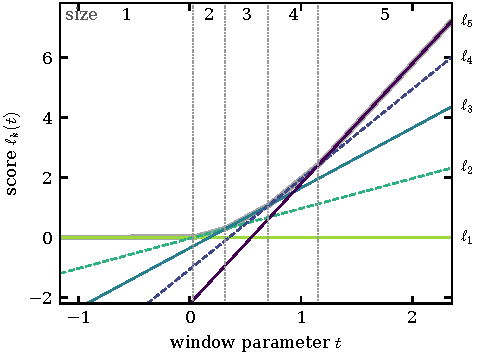
\includegraphics{figures/phases}
\caption{The lines~\eqref{eq:weakfield-lines} for $d=5$ and $h_i=-(i-1)^2$. The
gray band is their upper envelope. The dotted lines are $t_1<\cdots<t_4$, and
the number at the top of each interval is the size $k$ of the winning support
$\{1,\ldots,k\}$.}
\label{fig:phases}
\end{figure}


\section{Near the boundary of the simplex}
\label{sec:frontier-boundary}

So far every positive coordinate was of order $N$
(Theorem~\ref{thm:simplex-interior} needs each to be at least $\varepsilon N$).
What about bins with some small coordinates, near an edge or a vertex of the
triangle? In this section we drop that assumption. We first give an upper bound
that holds for every positive count vector (Theorem~\ref{thm:uniform-simplex-majorant}).
Then we find the scale at which a small coordinate starts to matter. It is
$N/L^2$ when at least 2 coordinates are of order $N$
(Remark~\ref{rem:crossover-scale}). Near a vertex the picture changes: the
crossing moves to odds of order $N^{-1/2}$, and the small coordinates alone
decide it (Subsection~\ref{sec:vertex-completion}).

The start is uniform, but note that $S_n(u)$ does not involve the start.
Proposition~\ref{prop:dpmf} gives
$P^\mu_N(n)\le(\max_i\mu_i)\,p^{N-1}S_n(u)$ for every start $\mu$, so every
upper bound below also holds for a general start. The basic tool compares the
Laguerre-type polynomials of the ratio form with the Bessel series $\Phi$.

\begin{lemma}[a uniform Laguerre--Bessel inequality]
\label{lem:uniform-laguerre-bessel}
For every integer $a\ge1$ and real $w>0$,
\begin{equation}\label{eq:uniform-laguerre-bessel}
0\le1-\frac{B_a(w)}{w\Phi(aw)}\le\frac w2,
\qquad
B_a(w)=\sum_{m=1}^{a}\binom{a-1}{m-1}\frac{w^m}{m!}.
\end{equation}
\end{lemma}

The proof, in Appendix~\ref{app:boundary}, compares coefficients with
Lemma~\ref{lem:clipped-product}.

\begin{theorem}[a uniform Bessel majorant on every simplex stratum]
\label{thm:uniform-simplex-majorant}
Let $n_1,\ldots,n_k$ be arbitrary positive integers with sum $N$, and let
$0<u<1$, $v=u/(1-u)$. Define
\[
\mathcal Q_n(u)=(1-u)^{N-1}v^{k-1}
\int_0^\infty e^{-t}t^k\prod_{i=1}^k\Phi(n_i vt)\,dt.
\]
Then, with no lower bound on any $n_i/N$,
\begin{equation}\label{eq:uniform-simplex-majorant}
0\le1-\frac{S_n(u)}{\mathcal Q_n(u)}
\le k(k+1)v+\frac{k}{2}v^2\left(\sum_i\sqrt{n_i}\right)^2
\le k(k+1)v+\frac{k^2}{2}Nv^2.
\end{equation}
Thus this approximation has relative error $O_k(L^2/N)$ whenever
$u=O(L/N)$, uniformly over every positive composition of $N$.
\end{theorem}

In words, $\mathcal Q_n$ is an upper bound for every bin, and it is sharp up to
a relative error $O(L^2/N)$ in the range of the crossings. Here is the idea of
the proof, which is in Appendix~\ref{app:boundary}. We apply
Lemma~\ref{lem:uniform-laguerre-bessel} to each factor of an integral form
of $S_n$. Then the relative error is at most $kv/2$ times the mean of $t$
under the probability density proportional to
$e^{-t}t^k\prod_i\Phi(n_ivt)$, and an integration by parts bounds this mean by
$2(k+1)+v(\sum_i\sqrt{n_i})^2$.

\begin{remark}[the scale $N/(\log N)^2$]\label{rem:crossover-scale}
Here is the heuristic. A small coordinate $a$ adds its own runs. Each run needs
about 2 switches, which gives a factor $u^2$, and it can go in about $N$ places.
So what matters is $aNu^2$. At the crossings of
Section~\ref{sec:simplex-thresholds} the value $Nu=T/p$ is of order $L$, and
then $aNu^2$ is of order $aL^2/N$. So when at least 2 coordinates are of order
$N$, a rare count starts to matter once it has size $\rho N/L^2$ with $\rho$
fixed.

Appendix~\ref{app:boundary} proves this. Take $k_1\ge2$ large coordinates with
fractions $\beta_i$ among themselves and $\ell$ rare counts
$a_j=\rho_jN/L^2$. With $z=Nu$,
Theorem~\ref{thm:simplex-boundary-crossover} gives $S_n(z/N)$ up to a factor
$1+O(L^{-2}+L^2/N)$. Each rare count contributes a factor
$\Phi(A^2a_jz^2/N)$, where $A=\sum_i\sqrt{\beta_i}$, and the complete
correction of relative order $1/L$ is a factor $e^{\mathcal E(z)}$ with 3
terms. The theorem also gives the crossing as the root of an implicit
equation, and as an explicit expansion in $L$, which converges slowly. Rare
counts with $a_j=o(N/L^2)$ change that expansion only by $o(1)$
(Corollary~\ref{cor:simplex-rare-invisibility}), but their number $\ell$
changes its leading and logarithmic coefficients. With only one large
coordinate the formula would have $A=1$, so the growth factor
$e^{(A^2-1)z}$ is gone. Then the crossing moves to $u$ of order $b^{-1/2}$,
where $b$ is the large count, and the scale changes. This is the case of
Subsection~\ref{sec:vertex-completion}.
\end{remark}

\subsection{Near a vertex}\label{sec:vertex-completion}

Now let one count $b$ be large and let the other positive counts
$a_1,\ldots,a_\ell$ be small compared with $b$, with $\ell\ge1$ fixed. In
this subsection and in Appendix~\ref{app:vertex} we put
$|a|=a_1+\cdots+a_\ell$. These rare counts are not the constants $a_k$ of
Section~\ref{sec:simplex-thresholds}, which do not appear here. With
$B_a$ as in Lemma~\ref{lem:uniform-laguerre-bessel}, put
\[
H(y)=\prod_{i=1}^{\ell}B_{a_i}(y),\qquad
\kappa(y)=\frac{yH'(y)}{H(y)}.
\]
The polynomial $H$ has positive coefficients, $H(0)=0$ and $H(1)\ge1$, so
$H(y_a)=1$ has exactly one positive root $y_a$, and $y_a\le1$. Write
$S_{(b,a)}$ for $S_n$ with $n=(b,a_1,\ldots,a_\ell)$. It is a polynomial in
$u$ with nonnegative coefficients, zero constant term and a positive
coefficient at $u^\ell$, so $S_{(b,a)}(u)=1$ has exactly one positive root
$u_{b,a}$.

Each rare run again needs about 2 switches and has about $b$ places, so the
rare counts enter through $bu^2$. For fixed rare counts the bounds of
Lemma~\ref{lem:vertex-randomization} in Appendix~\ref{app:vertex} give
$S_{(b,a)}(\sqrt{y/b})\to H(y)$ as $b\to\infty$. So the crossing is near
$\sqrt{y_a/b}$, and $Nu$ is of order $\sqrt N$ instead of $L$. The next
theorem shows that this leading term stays correct uniformly as long as
$|a|=o(b)$.

\begin{theorem}[all growing rare counts near a vertex]
\label{thm:vertex-uniform-root}
Fix $\ell\ge1$. Uniformly over all positive rare counts with $|a|=o(b)$, the
unique positive crossing odds satisfy
\begin{equation}\label{eq:vertex-uniform-root}
 u_{b,a}=\sqrt{\frac{y_a}{b}}
 \left(1+O_\ell\!\left(\sqrt{\frac{|a|+1}{b}}\right)\right),
 \qquad \prod_i B_{a_i}(y_a)=1.
\end{equation}
Explicitly, put
\[
 c_\ell=\ell+\sqrt\ell+1,\quad
 \varepsilon=\sqrt{\frac{|a|+1}{b}},\quad \delta=16c_\ell\varepsilon.
\]
If $\delta\le1/2$, then
\begin{equation}\label{eq:vertex-uniform-bracket}
 (1-\delta)\sqrt{y_a/b}\ \le u_{b,a}\le
 (1+\delta)\sqrt{y_a/b}.
\end{equation}
The constants are not optimized.
\end{theorem}

In words, near a vertex the crossing is decided by the polynomial $H$ of the
rare counts alone, evaluated at $bu^2$, as long as the rare counts have total
$o(b)$. The bracket~\eqref{eq:vertex-uniform-bracket} holds for all $b$ and all
positive rare counts with $\delta\le1/2$, and it
implies~\eqref{eq:vertex-uniform-root}.

The proof is in Appendix~\ref{app:vertex}. It rests on 2 facts. First,
$\log H$ is concave, and for $0<y\le1$ its elasticity $\kappa(y)$ lies
between $\max\{\ell,\frac12\sqrt{|a|y}\}$ and $\ell+\sqrt{\ell|a|y}$
(Lemma~\ref{lem:vertex-elasticity}). Second,
$S_{(b,a)}(u)=(1-u)^{|a|}\E[H(v\mathcal T)]$ exactly, where $v=u/(1-u)$ and
$\mathcal T$ is a gamma variable plus a compound binomial sum with mean
$2+(b-1)u$ (Lemma~\ref{lem:vertex-randomization}). Jensen's inequality then
gives $S_{(b,a)}(u)\ge(1-u)^{|a|}H(bu^2)$, which exceeds $1$ at
$u=(1+\delta)\sqrt{y_a/b}$. The tangent line of $\log H$ at $bu^2$ and the
moment generating function of $\mathcal T$ give an upper bound that is
below $1$ at $u=(1-\delta)\sqrt{y_a/b}$.

We have also found the next term of $u_{b,a}$ for fixed rare counts, which
for one rare count is the 2-state fixed-edge expansion of Paper~A, the growth
$u_{b,a}\sim\ell\log|a|/(2A\sqrt{|a|b})$ with $A=\sum_i\sqrt{a_i/|a|}$ when
$|a|\to\infty$ with proportions $a_i/|a|$ bounded away from $0$, and an example
with $|a|=o(b)$ where $S_{(b,a)}(u)\sim H(bu^2)$ fails although the root is
still correct (proofs omitted, checked numerically, see
Section~\ref{sec:verify}).


\section{Verification and open questions}\label{sec:verify}

{\sloppy
\paragraph{Data and code availability.}
No proof in this paper relies on computation. The code and the Lean files are
in the folder \nolinkurl{kagey-problems/problem131} of
\url{https://github.com/apemm/Kagey-Problems} (release
\texttt{paperB-arxiv-v1}). The checks for this paper are described in
\texttt{SUPPLEMENT.md}. The scripts are in the subfolder \texttt{paperB} and use
only the Python standard library. The command
\texttt{python -B verify\_all.py -{}-paper b} in \nolinkurl{kagey-problems/problem131}
runs all of them except \texttt{verify\_B\_tie\_repair.py}, which also runs
when \texttt{--full} is added. The scripts compare the exact law with dynamic
programs and with enumeration of all words, and check the crossings and the
constants. The statements marked as numerically verified are checked as
follows. For the error quoted after Proposition~\ref{prop:start-weights},
\texttt{verify\_general\_start.py} computes the start weights from the run form
and from the refresh form in double precision. For the finite-$N$ phases after
Example~\ref{ex:K3-start}, dynamic programs over all bins run at $N=90$ in
\texttt{verify\_general\_start.py} and at $N=300$ and $1002$ in
\texttt{verify\_B\_tie\_repair.py}. For Remark~\ref{rem:K3-finite} the two ends
of the window are found by bisection, at $N=300$ in
\texttt{verify\_B\_tie\_repair.py} and at $N\ge3000$ in
\texttt{verify\_general\_start.py}. The scripts
\texttt{verify\_frontier\_modes.py}, \texttt{verify\_frontier\_boundary.py} and
\texttt{verify\_vertex\_completion.py} check the field and the identities near
the boundary against word enumeration. The numbers in
Remark~\ref{rem:crossover-numbers} come from \texttt{verify\_crossover\_factor.py}.
For $N\le2\cdot10^6$ it computes $S_{(n,a)}$ in three ways, by the run form and
by a quadrature of~\eqref{eq:boundary-integral-form} in double precision and
by the sum~\eqref{eq:simplex-positive-sum} in 60-digit decimal arithmetic, and
for larger $N$ by the last two. They agree to about $10^{-14}$ in $\log S$.
None of these checks is interval-certified.

Many of the exact identities and finite bounds were also formalized in Lean~4,
in \nolinkurl{kagey-problems/problem131/lean/PaperB}, where \texttt{MAP.md}
matches each statement with its Lean theorem. These include the exact law for
the uniform start, balancing, the ordering of the constants $a_k$, most of the
arithmetic of Corollary~\ref{cor:weakfield-full-hierarchy}, and the bracket near
a vertex. The asymptotic results and the results for a nonuniform start were not
formalized.
\par}

\paragraph{Open questions.}
Several questions remain open. The discrete correction term
$-\frac{(k-1)^2}2z^2/N$ and the second-order ends of the window in
Remark~\ref{rem:K3-finite} are not proved. Neither is the failure of balancing
at every large $N$ for a start that is not constant on the face.
Corollary~\ref{cor:simplex-modes} has no effective $N_0$, and by
Example~\ref{ex:simplex-edge-mode} it does not extend to every $N$. Nothing is
said here about the modes when $T$ is much larger than $L$. Near a vertex the
leading crossing is known uniformly for rare counts of total $o(b)$, but neither
the next term uniformly in that range nor the case of a nonuniform start is
known. The crossover with a start that is not constant on the support, and a
number of states that grows with $N$, are also left open. Switching that is not
uniform is treated in a paper of the author that is in preparation.

\paragraph{Acknowledgment.} I thank Peter Kagey for posing the problem.

\section*{A note on the use of AI}
I wrote the proofs and derivations of Sections~2 and~3 by hand, without AI
assistance, before any revision. I then used Claude Opus 5.5 (Anthropic,
through Claude Code) in September and October 2026 to check everything I had
written for typos and for statements that were technically wrong. It found a
number of gaps, which I fixed, along with occasional wrong references and
unclear wording. I decided every revision and went over each one by hand. The model also
drafted rewordings of many passages, which I reviewed and edited. For the later sections I brainstormed
conjectures with the model, and several results came from it together with
proofs, namely the tree form of the constants in Proposition~\ref{prop:kirchhoff},
the start-law results (Lemma~\ref{lem:first-run},
Proposition~\ref{prop:start-weights}, Theorem~\ref{thm:start-maxima},
Corollary~\ref{cor:start-modes} and Example~\ref{ex:K3-start}) and the full
correction factor in Theorem~\ref{thm:simplex-boundary-crossover}. I rechecked
and rederived these proofs by hand. I also checked the proofs with GPT-6 Astra
(OpenAI), which found nothing beyond the earlier check.

The Lean~4 formalization in
\nolinkurl{kagey-problems/problem131/lean/PaperB} was generated by the
model, then revised and checked by hand against the corresponding results (see
\nolinkurl{MAP.md} in that folder). Parts of the Python verification scripts
were also written by the model, which cross-checked them against each other.
Lastly, I used it for literature search, namely to find and verify sources
beyond the ones I had first checked on my own.

All mathematical claims, proofs and computations in this paper are my
responsibility.

\section*{Statements and declarations}
\paragraph{Competing interests.} The author has no competing interests to
declare.

\paragraph{Funding.} No funding was received for this work.

\paragraph{Data availability.} All code, data and Lean files supporting this
paper are in the folder \nolinkurl{kagey-problems/problem131} of
\url{https://github.com/apemm/Kagey-Problems}, at the release
\texttt{paperB-arxiv-v1}. Section~\ref{sec:verify} describes what each check
does and how to rerun it.

\appendix
\section{\texorpdfstring{Proofs for Sections~\ref{sec:multistate-model}
and~\ref{sec:simplex-thresholds}}{Proofs for Sections 2 and 3}}\label{app:thresholds}

\subsection{Facts about Bessel series}

The weights $x^m/(m!(m+1)!)$ of the series $\Phi$ define a probability law on
the integers $m\ge0$. Its moments control every Laplace expansion in this
paper.

\begin{lemma}[the Bessel law]\label{lem:bessel-law}
For $x\ge0$ let $J$ be a random variable with
$\Prob(J=m)=x^m/[m!(m+1)!\,\Phi(x)]$ for $m\ge0$ (so $J=0$ when $x=0$), and put
$\psi(x)=\E J$. Then
\begin{enumerate}[(i)]
\item $\E[J(J+1)]=x$,
\item $\E[J(J-1)J(J+1)]=x^2$,
\item $\psi(x)=x\Phi'(x)/\Phi(x)$, and $\psi(x)=\sqrt x\,I_2(2\sqrt x)/I_1(2\sqrt x)$
for $x>0$,
\item $x\psi'(x)=\Var J$, so $0\le\psi'(x)\le1$ for $x>0$, and $\psi'(0)=\frac12$,
\item $0\le\psi(x)\le\min(x/2,\sqrt x)$,
\item $0\le(\log\Phi)'(x)=\psi(x)/x\le\frac12$ for $x>0$.
\end{enumerate}
\end{lemma}

\begin{proof}
(i) We have $\sum_{m\ge1}m(m+1)x^m/[m!(m+1)!]=\sum_{m\ge1}x^m/[(m-1)!m!]=x\Phi(x)$.
(ii) For $m\ge2$, $m(m-1)/m!=1/(m-2)!$ and $m(m+1)/(m+1)!=1/(m-1)!$, so the sum is
$\sum_{m\ge2}x^m/[(m-2)!(m-1)!]=x^2\Phi(x)$.
(iii) The first form is the definition of the mean. Termwise,
$\Phi'(x)=\sum_{i\ge0}x^i/[i!(i+2)!]=I_2(2\sqrt x)/x$ by the series of
$I_2$~\cite[Eq.~10.25.2]{dlmf}, which gives the second.
(iv) Since $\log\Prob(J=m)=m\log x-\log\Phi(x)$ plus a term free of $x$, we
have $x\frac d{dx}\log\Prob(J=m)=m-\psi(x)$. So $x\psi'(x)=\E[J(J-\psi)]=\Var J$,
and $\Var J\le\E J^2\le\E[J(J+1)]=x$. From the series,
$\psi(x)=x(\frac12+\frac x6+\cdots)/(1+\frac x2+\cdots)=\frac x2+O(x^2)$, so
$\psi'(0)=\frac12$.
(v) For integers $J\ge0$ we have $J\le J(J+1)/2$, so $\psi\le x/2$ by (i). Also
$\psi^2\le\E J^2\le x$.
(vi) follows from (iii) and (v).
\end{proof}

\begin{lemma}[clipped product deficit]\label{lem:clipped-product}
For any finite list of nonnegative real numbers $t_1,\ldots,t_m$, with
$(x)_+=\max(x,0)$,
\[
0\le1-\prod_{j=1}^m(1-t_j)_+\le\sum_{j=1}^mt_j.
\]
\end{lemma}

\begin{proof}
If some $t_j\ge1$, the product is zero and the sum is at least one. Otherwise all
factors lie in $[0,1]$, and induction on $m$ follows from
$1-(1-a)(1-b)=a+b-ab\le a+b$ for $a,b\in[0,1]$. The empty product gives
equality.
\end{proof}

\begin{lemma}[Gaussian averages of the factors $\Phi$]\label{lem:gaussian-phi-average}
Fix $q\ge0$, an integer $\ell\ge0$ and $X\ge0$. Let $w_0\ge1$ and
$c_1,\ldots,c_\ell\ge0$ with $\xi_j=c_jw_0^2\le X$, and put
$F(w)=w^q\prod_{j=1}^\ell\Phi(c_jw^2)$. Let $J_1,\ldots,J_\ell$ be independent,
with $J_j$ distributed as $J$ in Lemma~\ref{lem:bessel-law} with $x=\xi_j$. Put
$|J|=J_1+\cdots+J_\ell$ and $\mu_q=\E[(q+2|J|)(q+2|J|-1)]$. Then
\[
\frac1{\sqrt\pi}\int_{-w_0/2}^{w_0/2}e^{-y^2}F(w_0+y)\,dy
=F(w_0)\Bigl(1+\frac{\mu_q}{4w_0^2}+O(w_0^{-4})\Bigr),
\]
and $F(w_0+y)=O(F(w_0))$ for $|y|\le w_0/2$. The constants depend only on $q$,
$\ell$ and $X$. Moreover
\[
\mu_q=q^2-q+4\sum_j\xi_j+(4q-6)\sum_j\psi(\xi_j)
+8\sum_{i<j}\psi(\xi_i)\psi(\xi_j).
\]
\end{lemma}

\begin{proof}
\emph{Step 1. Derivatives as moments.} Expanding each $\Phi$ gives
$F(w)=\sum_m\kappa_mw^{q+2|m|}$, where $m=(m_1,\ldots,m_\ell)$ runs over vectors
of nonnegative integers, $|m|=\sum_jm_j$ and
$\kappa_m=\prod_jc_j^{m_j}/[m_j!(m_j+1)!]\ge0$. The weights
$\kappa_mw_0^{q+2|m|}/F(w_0)$ are the joint law of $(J_1,\ldots,J_\ell)$. Hence
$F^{(i)}(w_0)=F(w_0)\,\E[(q+2|J|)_i]\,w_0^{-i}$, where
$(y)_i=y(y-1)\cdots(y-i+1)$. In particular $F''(w_0)=\mu_qw_0^{-2}F(w_0)$.

\emph{Step 2. The fourth derivative.} Let $w=w_0+y$ with $|y|\le w_0/2$. For
every $\eta\ge0$ we have $w^{\eta-4}\le16(3/2)^\eta w_0^{\eta-4}$ (consider
$\eta\ge4$ and $\eta<4$ separately) and $|(\eta)_4|\le\eta^4+1$. Applying this
with $\eta=q+2|m|$ termwise gives
\[
|F''''(w)|\le16\Bigl(\frac32\Bigr)^qw_0^{q-4}
\prod_j\Phi\Bigl(\frac{9\xi_j}4\Bigr)\,
\tilde\E\bigl[(q+2|\tilde J|)^4+1\bigr],
\]
where the $\tilde J_j$ are independent with the parameters $9\xi_j/4$ in place of
$\xi_j$. By Lemma~\ref{lem:bessel-law}(i) and (ii),
$\E J^4=x^2+\E J^2\le x^2+x$. Hence $\tilde\E[(q+2|\tilde J|)^4]$ is bounded in
terms of $q$, $\ell$ and $X$. Since $\Phi\ge1$ we have $F(w_0)\ge w_0^q$, so
$F''''(w)=O(w_0^{-4}F(w_0))$. The same argument without derivatives bounds
$F(w_0+y)$.

\emph{Step 3. Taylor expansion.} Expand $F(w_0+y)$ to third order in $y$ with
the Lagrange remainder. The odd terms integrate to zero over the symmetric
interval. The integrals of $e^{-y^2}$ and $y^2e^{-y^2}$ over $|y|\le w_0/2$
differ from $\sqrt\pi$ and $\sqrt\pi/2$ by $O(w_0e^{-w_0^2/4})$, the number
$\mu_q$ is bounded, and the remainder term is $O(w_0^{-4}F(w_0))$. This proves
the expansion.

\emph{Step 4. The formula for $\mu_q$.} Put $\psi_j=\psi(\xi_j)=\E J_j$. Then
$\E J_j^2=\xi_j-\psi_j$ by Lemma~\ref{lem:bessel-law}(i), and independence gives
$\E[(q+2|J|)^2]=q^2+4q\sum_j\psi_j+4\sum_j(\xi_j-\psi_j)+8\sum_{i<j}\psi_i\psi_j$.
Subtracting $\E[q+2|J|]=q+2\sum_j\psi_j$ proves it.
\end{proof}

\subsection{Proofs for Section~\ref{sec:simplex-thresholds}}

\begin{proof}[Proof of the exact assertions in Theorem~\ref{thm:simplex-crossing}]
Let $n$ be a balanced vector with $k$ positive coordinates, so that
$C_{N,k}/V_N=S_n(u)$ with $u=(1-p)/((d-1)p)$.

\emph{Step 1. One crossing.} To count $W_n(j)$, choose a sequence of $j+1$ run
colors in which successive colors differ. If color $i$ appears $m_i$ times, its
run lengths can be chosen in $\binom{n_i-1}{m_i-1}$ ways. So every coefficient
of $S_n$ is nonnegative, and the first nonzero one is $W_n(k-1)=k!$, from the
$k!$ orders of $k$ single runs. Hence $S_n$ increases strictly from $0$ to
$\infty$ on $u>0$ and equals $1$ exactly once. As $p$ increases over $(0,1)$,
$u$ decreases over $(0,\infty)$, which gives the unique $p_{N,k}$ and the two
inequalities.

\emph{Step 2. Monotonicity in $N$.} Choose the balanced vectors for increasing
$N$ by adding $1$ to one of the smallest coordinates. Each coefficient $W_n(j)$
is then nondecreasing. To see this, map a word to the word with an extra copy of
the incremented color just before its first occurrence. This keeps the number
of changes, and it is injective, since deleting the first letter of the first
run of that color inverts it. The coefficient of $u^k$ is
\[
W_n(k)=\frac{k!(k-1)}2\sum_i(n_i-1)=\frac{k!(k-1)}2(N-k).
\]
Indeed, exactly one run color appears twice. For each choice of it there are
$(k+1)!/2-k!=k!(k-1)/2$ sequences of run colors in which successive colors
differ (all orders, minus those with the two copies adjacent), and $n_i-1$ ways to
split its $n_i$ visits into two runs. This coefficient increases strictly with
$N$. So at every $u>0$ the value $S_n(u)$ increases strictly with $N$, the root
of $S_n(u)=1$ decreases strictly with $N$, and $p=1/(1+(d-1)u)$ increases.

\emph{Step 3. The first crossing.} If $N=k$, every coordinate is $1$ and
$S_n(u)=k!u^{k-1}$, which gives $p_{k,k}$. Since the root decreases with $N$,
every root has $u\le(k!)^{-1/(k-1)}<1$, and $u<1$ means $r<p$, that is,
$p>1/d$.
\end{proof}

The asymptotic assertions rest on a Laplace expansion of the positive
sum~\eqref{eq:simplex-positive-sum}. It is the case with no rare counts of the
crossover theorem in Appendix~\ref{app:boundary}.

\begin{lemma}[no rare counts]\label{lem:no-rare}
Fix $k\ge2$, $\varepsilon>0$ and $0<c<C$. Let $n$ be a positive count vector
with $k$ coordinates and total $N$, put $\beta=n/N$, and assume that every
$\beta_i\ge\varepsilon$. Put $A=\sum_i\sqrt{\beta_i}$, $g=A^2-1$ and $s=k-1$,
let $D(\beta)$ be as in Theorem~\ref{thm:simplex-interior}, and put
\[
\gamma_0(\beta)=\frac{k(k+2)}{16A^2}-\frac3{16A}\sum_{i=1}^k\beta_i^{-1/2}.
\]
Then, uniformly for these $n$ and $cL\le z\le CL$,
\begin{equation}\label{eq:no-rare}
S_n(z/N)=D(\beta)\frac{z^{s/2}e^{gz}}{N^s}\,e^{\gamma_0(\beta)/z}
\Bigl(1+O\Bigl(\frac1{L^2}+\frac{L^2}N\Bigr)\Bigr).
\end{equation}
\end{lemma}

\begin{proof}
This is Theorem~\ref{thm:simplex-boundary-crossover} with $\ell=0$ and $k_1=k$.
Then $M=N$, $\eta=s/2$, the constant $D_{k_1}(\beta)$ is $D(\beta)$, there are
no factors $\Phi$, and $\mathcal E(z)=\gamma_0/z$ with $\gamma_0$ as above,
since $(2\eta+1)(2\eta+3)=k(k+2)$. The proof of that theorem uses only
Theorem~\ref{thm:uniform-simplex-majorant}, the expansion of $I_1$ and
Lemma~\ref{lem:gaussian-phi-average}, and nothing from
Section~\ref{sec:simplex-thresholds}.
\end{proof}

\begin{proof}[Proof of the asymptotic assertions in
Theorems~\ref{thm:simplex-window} and~\ref{thm:simplex-crossing}]
Put $s=k-1$ and let $n$ be balanced, so that $\beta_i=n_i/N=1/k+O(1/N)$.

\emph{Step 1. The balanced ratio~\eqref{eq:simplex-uniform-ratio}.} At the
center $A^2-1=s$, $D(\beta)=D_k$ and $\gamma_0=(k+2)/16-3k/16=-s/8$. On the
plane $\sum_i\beta_i=1$ the function $A^2$ has a critical point at the center,
so $A^2-1=s+O(N^{-2})$, while $D(\beta)$ and $\gamma_0(\beta)$ change by
$O(1/N)$. Since $z=O(L)$, Lemma~\ref{lem:no-rare} with $\varepsilon=1/(2k)$ and
$e^{-s/(8z)}=1-s/(8z)+O(z^{-2})$ gives~\eqref{eq:simplex-uniform-ratio}.

\emph{Step 2. Parts (i) to (iii).} Let $cL\le T\le CL$ and $u=r/p$, so that
$z=T/p$ lies in $[cL,2CL]$ for large $N$ and $z-T=(d-1)Tz/N=O(L^2/N)$. Take
logarithms in~\eqref{eq:simplex-uniform-ratio}, with $c$ and $2C$ in place of $c$
and $C$, and replace $z$ by $T$. This changes each term by $O(T^2/N)$, and
$\log D_k=-sa_k$, so we get (i). For (ii),
$\log V_N=(N-1)\log(1-(d-1)T/N)-\log d=-(d-1)T-\log d+O(T^2/N)$. With $T=\tau L$
and (i) we get $\log C_{N,k}=-(d-1)\tau L+(k-1)(\tau-1)L+O(\log L)$, which is (ii),
and the case $k=1$ is the formula for $\log V_N$. For (iii),
$T=L-\frac12\log L+t$ gives $\Psi_N(T)=t+\frac12\log(T/L)=t+O(\log L/L)$
uniformly on compact $t$ sets, and the terms $1/(8T)$ and the error tend to $0$.

\emph{Step 3. The crossing.} Part (i) at $T=L/2$ and at $T=2L$ shows that the
ratio tends to $0$ and to $\infty$. Since $S_n(u)$ increases with $u$ and $u$
increases with $T$, the root lies in $[L/2,2L]$ for large $N$, and (i) applies
there with $c=\frac12$ and $C=2$. The same argument at $T=(1\pm\varepsilon)L$
gives $T_{N,k}/L\to1$. At the root the left side of (i) is $0$, and dividing by
$s$ gives the implicit equation, since $T^2/N=o(L^{-2})$. For the explicit form
put $z_*=L-\frac12\log L+a_k+e_L/L$ with $e_L=\frac14\log L-\frac12a_k+\frac18$.
Since $\log z_*=\log L-\frac{\log L}{2L}+\frac{a_k}L+O(\frac{(\log L)^2}{L^2})$,
we get $z_*+\frac12\log z_*-1/(8z_*)=L+a_k+O((\log L)^2/L^2)$. The derivative of
$z+\frac12\log z-1/(8z)$ is at least $1$ for $z>0$, so
$T_{N,k}-z_*=O((\log L)^2/L^2)$, which is~\eqref{eq:simplex-root-expansion}.

\emph{Step 4. Part (iv).} We have $a_k=\frac12\log(4\pi)-f(k)$ with
$f(x)=(x+\frac12)\log x/(x-1)$. For $x\ge2$ the sign of $f'(x)$ is the sign of
$\Delta(x)=2x^2-x-1-3x\log x$. Here $\Delta(2)=5-6\log2>0$, and
$\Delta'(x)=4x-4-3\log x>0$ for $x\ge2$, since $\Delta'(2)>0$ and
$\Delta''(x)=4-3/x>0$. So $f$ increases strictly and $a_k$ decreases strictly.
\end{proof}

\begin{proof}[Proof of Theorem~\ref{thm:simplex-interior}]
The polynomial $S_n$ has nonnegative coefficients and lowest term $k!u^{k-1}$,
so $S_n(u)=1$ has a unique positive root. Lemma~\ref{lem:no-rare} with
$\beta=\alpha$ gives~\eqref{eq:simplex-interior-ratio}, since $\gamma_0(\alpha)$
is bounded when every $\alpha_i\ge\varepsilon$ and $e^{\gamma_0/z}=1+O(1/z)$.

For the root, note that $A^2=1+2\sum_{i<j}\sqrt{\alpha_i\alpha_j}$, so
$g\in[2\varepsilon,s]$, and $D(\alpha)$ has positive lower and finite upper
bounds depending on $k$ and $\varepsilon$. Put $c_0=\frac12$ and
$C_0=s/\varepsilon$. By~\eqref{eq:simplex-interior-ratio},
$\log S_n(c_0L/N)\le(gc_0-s)L+O(\log L)\le-\frac s2L+O(\log L)<0$ and
$\log S_n(C_0L/N)\ge(gC_0-s)L+O(\log L)\ge sL+O(\log L)>0$ for large $N$. So the
root has $Nu_n\in[c_0L,C_0L]$, and taking logarithms
in~\eqref{eq:simplex-interior-ratio} there gives
\[
gz+\frac s2\log z=sL-\log D(\alpha)+O_{k,\varepsilon}(z^{-1}+z^2/N),
\qquad z=Nu_n.
\]
First $z=(s/g)L+O_{k,\varepsilon}(\log L)$. Then
$\frac s2\log z=\frac s2\log L+\frac s2\log(s/g)+O(\log L/L)$, and solving for
$z$ gives~\eqref{eq:simplex-interior-root}. The derivative of the left side is
at least $g\ge2\varepsilon$, so the error is preserved on inversion. Finally,
the functions of $\alpha$ in the formula have bounded derivatives on the set
$\{\alpha_i\ge\varepsilon/2\}$. So moving $\alpha$ by $O(1/N)$ changes the
expression by $O(L/N)$, which the error term absorbs.
\end{proof}

\begin{proof}[Proof of Lemma~\ref{lem:occupation-covariance}]
Note that $(\mathcal Lx)_i=\sum_jc_{ij}(x_i-x_j)$ and $\mathcal L\mathbf1=0$. Take
$\theta$ with $\theta_1=0$ and put $\zeta=\operatorname{diag}(\varpi)f$. Then
$\sum_i\zeta_i=0$, $\mathcal L\chi=\zeta$ and the form is $2\zeta^\top\chi$. The
vector $\tilde\chi=\chi-\chi_1\mathbf1$ also solves $\mathcal L\tilde\chi=\zeta$,
with $\zeta^\top\tilde\chi=\zeta^\top\chi$ and $\tilde\chi_1=0$. So rows $2$ to
$k$ give $\mathcal L_{(1)}\tilde\chi'=\zeta'$, where primes delete the first
coordinate, and the form is $2\zeta'^\top\mathcal L_{(1)}^{-1}\zeta'$. As
$\theta_1=0$, we have $\zeta'=(D'-\varpi'\varpi'^\top)\theta'$ with
$D'=\operatorname{diag}(\varpi_2,\ldots,\varpi_k)$. Hence
$\Sigma=2(D'-\varpi'\varpi'^\top)\mathcal L_{(1)}^{-1}(D'-\varpi'\varpi'^\top)$. The
matrix determinant lemma gives
$\det(D'-\varpi'\varpi'^\top)=\prod_{i\ge2}\varpi_i\,(1-\sum_{i\ge2}\varpi_i)=\prod_i\varpi_i$,
and the matrix-tree theorem gives $\det\mathcal L_{(1)}=\tree(c)>0$. For
nonnegative integer $c_{ij}$ this is the matrix-tree theorem for
multigraphs~\cite{bollobas1998}. Both sides are polynomials in the $c_{ij}$, so
they agree for all real $c_{ij}$.
\end{proof}

\begin{proof}[Proof of Proposition~\ref{prop:kirchhoff}]
(1) For $i\ne j$ we have $\alpha_iG^\alpha_{ij}=\phi_i\phi_j$, which is symmetric, so
$\alpha$ is reversible and hence stationary. Also $(Q_k\phi)_i=A-k\phi_i$, so
$\theta_{\alpha,i}=k-A/\phi_i$, and $Q_k+\operatorname{diag}(\theta_\alpha)$ has
off-diagonal entries $1$ and diagonal entries $1-A/\phi_i$. It is symmetric and
kills $\phi>0$, so $0$ is its Perron root. Conjugating by $\operatorname{diag}(\phi)$
gives the rates $\phi_j/\phi_i$. If $G^\alpha$ were a Doob transform of $Q_k$, then $\phi$
would be an eigenvector of $Q_k$, so $A-k\phi_i=\lambda\phi_i$ for all $i$ and $\alpha$
would be uniform.
(2) is Lemma~\ref{lem:weighted-cayley} with $x_i=\phi_i$.
(3) By (2), $\sqrt{\tree(\alpha)}/\prod_i\alpha_i=(\prod_i\alpha_i)^{-3/4}A^{k/2-1}$,
which gives the first form. Lemma~\ref{lem:occupation-covariance} with $\varpi=\alpha$
gives $\det(2\pi\Sigma_\alpha)=(4\pi)^{k-1}(\prod_i\alpha_i)^2/\tree(\alpha)$, which
gives the second.
(4) At the center $\mathcal L_{(1)}=I-J/k$ and $D'-\alpha'\alpha'^\top=(I-J/k)/k$
in the formula $\Sigma=2(D'-\alpha'\alpha'^\top)\mathcal L_{(1)}^{-1}
(D'-\alpha'\alpha'^\top)$ from the proof of
Lemma~\ref{lem:occupation-covariance}. This gives $\Sigma_k$. Substituting
$\tree(\alpha)=1/k$ and $\prod_i\alpha_i=k^{-k}$ into (3) gives $D_k$.
(5) is the same computation with $k_1$ and $\beta$.
\end{proof}

\begin{proof}[Proof of Proposition~\ref{prop:mass-balance}(2) and (3)]
Let $u=z/N$ with $cL\le z\le CL$, and put $s=k-1$.

\emph{Step 1. The mass.} In (1) the term $j=k$ is
$k(1+(k-1)z/N)^{N-1}=k\,e^{(k-1)z+O(z^2/N)}$, and each term with $j<k$ is smaller
by a factor $O(e^{-z})$. This gives the first expression.

\emph{Step 2. The Hessian.} Write $\alpha'=(\alpha_2,\ldots,\alpha_k)$ and
$g(\alpha)=A^2-1$ as in Theorem~\ref{thm:simplex-interior}. In full coordinates
the Hessian of $A^2$ at the center is $(k/2)J-(k^2/2)I$. Pulling it back along
$w=(-\sum_iv_i,v)$ gives $-\nabla^2g=(k^2/2)(I+J)$ in the coordinates
$\alpha'$, and its inverse is $(2/k^2)(I-J/k)=\Sigma_k$.

\emph{Step 3. The bins near the center.} Fix a small $\eta>0$ and let $K_\eta$ be
the set of $\alpha$ with $|\alpha_i-1/k|\le\eta$ for all $i$. On $K_\eta$,
Theorem~\ref{thm:simplex-interior} gives
$S_n=D(\alpha)z^{s/2}e^{g(\alpha)z}N^{-s}(1+O(z^{-1}+z^2/N))$ uniformly, with
$\alpha=n/N$. The points $\alpha'$ form a lattice with cells of volume $N^{-s}$,
and on each cell $g$ changes by $O(1/N)$ and $D$ by a factor $1+O(1/N)$. So the
sum over $n/N\in K_\eta$ is $N^s$ times the integral of the same expression over
$K_\eta$, times $1+O(z/N)$, up to the cells near the boundary of $K_\eta$. There
$g\le k-1-c_\eta$ for some $c_\eta>0$, so these cells are negligible. The function
$g$ has its strict maximum $k-1$ at the center, and $D$ is continuous there with
$D=D_k$. So Laplace's method gives
\[
\int_{K_\eta}D(\alpha)e^{g(\alpha)z}\,d\alpha'
=D_ke^{(k-1)z}\Bigl(\frac{2\pi}z\Bigr)^{s/2}(\det\Sigma_k)^{1/2}(1+o(1)).
\]
Multiplied by $z^{s/2}$ this is the second expression, provided the bins off
$K_\eta$ are negligible.

\emph{Step 4. The other bins.} For them, Theorem~\ref{thm:uniform-simplex-majorant}
and $\Phi(x)\le e^{2\sqrt x}$ give, with $Y=Nv$ and $A_n=\sum_i\sqrt{n_i/N}$,
\[
S_n(u)\le(1-u)^{N-1}v^s\int_0^\infty e^{-t+2A_n\sqrt{Yt}}\,t^k\,dt
\le C'\,\frac{(1+z)^{2k}}{N^s}\,e^{(A_n^2-1)z+O(z^2/N)},
\]
where we wrote $-t+2A_n\sqrt{Yt}=A_n^2Y-(\sqrt t-A_n\sqrt Y)^2$. Here
$A_n^2\le k-c'_\eta$ for some $c'_\eta>0$, since $A^2$ is continuous on the
closed simplex and equals $k$ only at the center. There are at most $N^s$ bins,
so they contribute $O(z^{2k}e^{(k-1-c'_\eta)z})=o(e^{(k-1)z})$. This proves (2).

\emph{Step 5. Part (3).} Equate the two expressions in (2) and let $N\to\infty$.
This gives $k=D_k(2\pi)^{s/2}(\det\Sigma_k)^{1/2}$, that is,
$D_k=k\det(2\pi\Sigma_k)^{-1/2}$. As a check,
$\det\bigl((k^2/2)(I+J)\bigr)=(k^2/2)^sk$, which gives
$D_k=k^{k+1/2}(4\pi)^{-s/2}$ again.
\end{proof}

\begin{proof}[Proof of Theorem~\ref{thm:simplex-balance}]
At $p=1/d$ the chain is a sequence of independent uniform states, and by the
multinomial formula the move multiplies the probability by $n_b/(n_a+1)>1$. For $1/d<p<1$ we have $\sigma>0$ and $v=r/\sigma>0$.

\emph{Step 1. An integral form.} Writing $M!=\int_0^\infty e^{-t}t^M\,dt$ in the
uniform case of Proposition~\ref{prop:dpmf}(a) gives
\begin{equation}\label{eq:simplex-balance-integral}
P_N(n)=\frac{\sigma^{N-1}}{dv}\int_0^\infty e^{-t}
\prod_iB_{n_i}(vt)\,dt,\qquad
B_n(y)=\sum_{m=1}^n\binom{n-1}{m-1}\frac{y^m}{m!},
\end{equation}
where the product runs over the positive coordinates.

\emph{Step 2. Log-concavity.} We show that for each $y>0$ the sequence $B_n(y)$,
$n\ge1$, is strictly log-concave. Write
\[
\frac{B_n(y)}y=b_{n-1},\qquad
b_j=\sum_{i=0}^j\binom ji a_i,\quad
a_i=\frac{y^i}{(i+1)!},\qquad
c_j=\sum_{i=0}^j\binom ji a_{i+1}.
\]
Pascal's identity gives $b_{j+1}=b_j+c_j$. The ratio $c_j/b_j$ is the mean of the
strictly decreasing sequence $f_i=a_{i+1}/a_i=y/(i+2)$ under the weights
$\lambda_i=\binom jia_i$, $0\le i\le j$, normalized. Let $\lambda'_i=\binom{j+1}ia_i$,
$0\le i\le j+1$, be the weights for $j+1$, and put $\lambda_{j+1}=0$. On
$0\le i\le j$ the ratio $\lambda'_i/\lambda_i=(j+1)/(j+1-i)$ increases in $i$. So for
$i<l$ we have $\lambda'_i\lambda_l-\lambda'_l\lambda_i\le0$, with strict inequality when
$l=j+1$. Hence
\[
\sum_i\lambda'_if_i\sum_l\lambda_l-\sum_i\lambda'_i\sum_l\lambda_lf_l
=\sum_{i<l}(\lambda'_i\lambda_l-\lambda'_l\lambda_i)(f_i-f_l)<0,
\]
since $f_i>f_l$ for $i<l$. So the mean decreases strictly, $c_{j+1}/b_{j+1}<c_j/b_j$,
and $b_{j+1}/b_j=1+c_j/b_j$ decreases strictly with $j$. This is the strict
log-concavity. Since $B_n(y)=(y/n)L^{(1)}_{n-1}(-y)$, it is a Tur\'an-type
inequality for the Laguerre polynomials $L^{(1)}_{n-1}(-y)$.

\emph{Step 3. The transfer.} Let $b\ge a+2$. It follows that
$B_{a+1}(y)/B_a(y)>B_b(y)/B_{b-1}(y)$, that is,
$B_{a+1}(y)B_{b-1}(y)>B_a(y)B_b(y)$. Apply this
for $y=vt>0$ in~\eqref{eq:simplex-balance-integral} and integrate. So the move
strictly increases $P_N(n)$. Repeated moves reach a balanced bin from any bin
with the same support, and all balanced bins with this support have the same
probability by symmetry. This proves the theorem.
\end{proof}

\begin{proof}[Proof of Corollary~\ref{cor:simplex-modes}]
For large $N$, $T\le CL$ forces $r\to0$ and so $p>1/d$. By
Theorem~\ref{thm:simplex-balance} every global mode is a vertex or a balanced
bin, and all balanced bins with the same number of positive coordinates have the
same probability. So we compare the ratios $C_{N,k}/V_N=S_n(u)$, $2\le k\le d$,
with $1$ and with each other. Fix $0<c<1$.

\emph{Case $T\le cL$.} The ratio $S_n(u)$ increases with $u$, and $u$ increases
with $T$. So it is at most its value at $T=cL$, which is
$\exp(-(k-1)(1-c)L+O(\log L))\to0$ by Theorem~\ref{thm:simplex-window}(i). So the
vertices are the only modes, and $p>p_{N,d}$.

\emph{Case $cL\le T\le CL$.} Theorem~\ref{thm:simplex-window}(i) gives
$\log(C_{N,k}/V_N)=(k-1)(\Psi_N(T)-a_k)+o(1)$, uniformly. Fix $\delta>0$, with
$\delta<(a_{d-1}-a_d)/2$ when $d\ge3$. This is possible since $a_2>\cdots>a_d$.
If $\Psi_N(T)\le a_d-\delta$, every face ratio is at most
$e^{-(k-1)\delta+o(1)}<1$, so only the vertices are modes. If
$\Psi_N(T)\ge a_d+\delta$, the full center beats the vertices, and it beats a
balanced bin with $2\le k<d$ positive coordinates by
\[
(d-k)(\Psi_N(T)-a_d)+(k-1)(a_k-a_d)+o(1)>0 .
\]
If $|\Psi_N(T)-a_d|<\delta$, a proper face with $k\ge2$ states has
$(k-1)(\Psi_N(T)-a_k)+o(1)\le-(k-1)\delta+o(1)<0$, since $a_k-a_d>2\delta$. So it
loses to the vertices, and the comparison of the vertices with the full centers
is decided by the unique crossing $p_{N,d}$ of Theorem~\ref{thm:simplex-crossing}.
In each subcase the conclusion agrees with (i) to (iii).

The last claim follows from~\eqref{eq:simplex-root-expansion} and
$p_{N,k}=1-(d-1)T_{N,k}/N$, since $a_2>\cdots>a_d$.
\end{proof}

\section{\texorpdfstring{Proofs for Sections~\ref{sec:general-start}
and~\ref{sec:frontier-modes}}{Proofs for the start and the field}}\label{app:start-field}

\subsection{The start weights}

We prove Lemma~\ref{lem:start-weights} and
Proposition~\ref{prop:start-weights}. Throughout $1/d<p<1$, so $\sigma=p-r>0$
and $v=r/\sigma=u/(1-u)$. The refresh form in Proposition~\ref{prop:dpmf}(a) is
linear in $\mu$, and with $\mu=\delta_a$ it gives $p^{N-1}S^{(a)}_n(u)$. So, with
sums over $1\le m_b\le n_b$ for $b\in F$ and $M=\sum_bm_b$,
\begin{equation}\label{eq:startw-weights}
 \omega_a(n)=\E_w\Bigl[\frac{m_a}M\Bigr],\qquad
 w(m)\propto\frac{M!}{\prod_bm_b!}\,v^M\prod_{b\in F}\binom{n_b-1}{m_b-1}.
\end{equation}
So $\omega_a(n)$ is the mean fraction of the blocks of the refresh form
that carry state $a$.

\begin{proof}[Proof of Lemma~\ref{lem:start-weights}]
(1) Exchanging the letters $a$ and $b$ is a bijection from the words with counts
$n$ that start with $a$ to those that start with $b$. It keeps the counts, since
$n_a=n_b$, and the number of changes, so $S^{(a)}_n=S^{(b)}_n$. If $k$ divides
$N$, a balanced $n$ has equal coordinates, and the $k$ weights are equal and sum
to $1$.

(2) We may take $N\ge N_0$ so large that $p>1/d$ and $\sigma\ge\frac12$. Let $n$
be balanced and $\nu=\lfloor N/k\rfloor$, so each $n_b$ is $\nu$ or $\nu+1$, and
$\nu\ge N/(2k)$.

\emph{Step 1. Reduction to two values.} By (1) the weights take a value $\omega_+$
where $n_b=\nu+1$ and a value $\omega_-$ where $n_b=\nu$. We show that
$0\le\omega_+-\omega_-\le\delta$ with $\delta=\frac2\nu(\E_wM+\E_wM^2)$. Since
the weights average to $1/k$, each is then within $\delta$ of $1/k$, and
$|\sum_a\mu_a\omega_a(n)-\mu(F)/k|\le\mu(F)\delta$.

\emph{Step 2. Pairing.} Let $n_a=\nu+1$ and $n_b=\nu$, and let $m'$ be $m$ with
$m_a$ and $m_b$ exchanged, with $w(m')=0$ if $m'$ is not admissible. All factors
of $w(m)$ other than $\binom{\nu}{m_a-1}\binom{\nu-1}{m_b-1}$ are symmetric in
$m_a$ and $m_b$. From $\binom\nu j/\binom{\nu-1}j=\nu/(\nu-j)$ we get
$w(m')=w(m)(\nu-m_a+1)/(\nu-m_b+1)$ when $m_a\le\nu$, and $w(m')=0$ when
$m_a=\nu+1$. In both cases $w(m)-w(m')=w(m)(m_a-m_b)/(\nu-m_b+1)$ when
$m_a>m_b$. The map $m\mapsto m'$ matches the admissible $m$ with $m_a<m_b$ to
the admissible $m$ with $m_b<m_a\le\nu$. Pairing $m$ with $m'$
in~\eqref{eq:startw-weights} gives, with $Z=\sum_mw(m)$,
\[
 \omega_a-\omega_b=\frac1Z\sum_{m_a>m_b}\bigl(w(m)-w(m')\bigr)\frac{m_a-m_b}M
 =\frac1Z\sum_{m_a>m_b}w(m)\frac{(m_a-m_b)^2}{M(\nu-m_b+1)}\ge0.
\]
Here $(m_a-m_b)^2/M\le M$. If $m_b\le\nu/2$ the last factor is at most $2/\nu$. If
$m_b>\nu/2$, then $M>\nu/2$ and the term is at most $w(m)M<w(m)\,2M^2/\nu$. This
proves the bound $\delta$.

\emph{Step 3. The moments.} It remains to bound $\E_wM$ and $\E_wM^2$. Since
$(m-1)!\binom{n_b-1}{m-1}/n_b^{m-1}=\prod_{j<m}(1-j/n_b)_+$, we have
$w(m)\propto c(m)A(m)$ for all $m$ with every $m_b\ge1$, where
\[
 c(m)=M!\prod_b\frac{(n_bv)^{m_b}}{m_b!(m_b-1)!},\qquad
 A(m)=\prod_b\prod_{j<m_b}\Bigl(1-\frac j{n_b}\Bigr)_+\in[0,1],
\]
and Lemma~\ref{lem:clipped-product} gives $1-A(m)\le\sum_bm_b^2/(2n_b)\le M^2/\nu$.
Write $M!=\int_0^\infty e^{-t}t^M\,dt$. Since
$\sum_{m\ge1}y^m/(m!(m-1)!)=y\Phi(y)$, this gives
$\E_c[(M+1)(M+2)]=\langle t^2\rangle$, where $\langle\cdot\rangle$ is the mean
under the density proportional to $e^{-t}t^k\prod_b\Phi(n_bvt)$, as in the
proof of Theorem~\ref{thm:uniform-simplex-majorant}. The integration by parts
there, with $t^{k+2}$ in place of $t^{k+1}$, gives
$\langle t^2\rangle=(k+2)\langle t\rangle+\sum_b\langle t\psi(n_bvt)\rangle$. Put
$c_1=\sqrt v\sum_b\sqrt{n_b}$. That proof gives
$\langle t\rangle\le2(k+1)+c_1^2$, and $\psi(x)\le\sqrt x$ and
$\langle t^{3/2}\rangle\le\langle t^2\rangle^{3/4}$ give
$X=\langle t^2\rangle\le(k+2)(2k+2+c_1^2)+c_1X^{3/4}$. If $c_1X^{3/4}\ge X/2$,
then $X\le16c_1^4$, and otherwise $X\le2(k+2)(2k+2+c_1^2)$. So
$X\le C_2(1+c_1^2)^2$, where $C_2$ depends only on $k$. Here
$c_1^2\le kNv=kT/\sigma\le2kT\le2kCL$, so
$\E_cM^2\le\E_c[(M+1)(M+2)]\le\nu/2$ for $N\ge N_0$. Since $0\le A\le1$ and
$\E_c[A]\ge1-\E_cM^2/\nu\ge\frac12$, and $M\le M^2$,
\[
 \E_wM\le\E_wM^2=\frac{\E_c[M^2A]}{\E_c[A]}
 \le\frac{\E_cM^2}{1-\E_cM^2/\nu}\le2C_2(1+2kT)^2.
\]
With $\nu\ge N/(2k)$ this gives $\delta\le C_1(1+T)^2/N$.
\end{proof}

\begin{proof}[Proof of Proposition~\ref{prop:start-weights}]
Take $N$ large, so that $0<u<1$ and $z=Nu\in[cL,2CL]$. Let $k=|F|$, put
$s=k-1$, $\Sigma=\sum_{b\in F}\sqrt{n_b}=A\sqrt N$ and
$\lambda=u(A/\sqrt{\alpha_a}-1)$. Note that
$A/\sqrt{\alpha_a}-1=\sum_{b\ne a}\sqrt{\alpha_b/\alpha_a}$ lies in
$[\sqrt\varepsilon,s/\sqrt\varepsilon]$. Let $j_1=\lfloor N/\sqrt L\rfloor$, so
that $j_1\le\varepsilon N/2$ for large $N$. We split the sum of
Lemma~\ref{lem:first-run} at $j_1$. The constants below depend only on $d$,
$k$, $\varepsilon$, $c$ and $C$.

\emph{Step 1. One term.} Let $1\le j\le j_1$, and put $n'=n-je_a$, $N'=N-j$ and
$\alpha'=n'/N'$. Then every $\alpha'_b\ge\varepsilon/2$,
$|\alpha'-\alpha|\le2\sqrt k\,j/N$ and $N'u\in[z/2,z]$. Since $N'\ge N/2$, for
large $N$ both $N'u$ and $z$ lie between $\frac c2\log N'$ and $4C\log N'$. So
Theorem~\ref{thm:simplex-interior}, with $\varepsilon/2$ in place of
$\varepsilon$ and with the constants $\frac c2$ and $4C$, applies at the totals
$N'$ and $N$ with errors $O(1/L)$. The difference of its exponents is
$(A(\alpha')^2-1)N'u-(A^2-1)z=u(\Sigma'^2-\Sigma^2)+ju$, where
$\Sigma'=\Sigma-\delta$ and
$\delta=\sqrt{n_a}-\sqrt{n_a-j}=j/(\sqrt{n_a}+\sqrt{n_a-j})$. So
$\delta\le j/\sqrt{n_a}$, and
\[
 0\le\delta-\frac j{2\sqrt{n_a}}
 =\frac{j\delta}{2\sqrt{n_a}\,(\sqrt{n_a}+\sqrt{n_a-j})}
 \le\frac{j^2}{2n_a^{3/2}}.
\]
Since $\Sigma\le\sqrt{kN}$ and $n_a\ge\varepsilon N$, this gives
$u(\Sigma'^2-\Sigma^2)=-2u\Sigma\delta+u\delta^2=-juA/\sqrt{\alpha_a}
+O(zj^2/N^2)$. Also $D(\alpha')/D(\alpha)=1+O(j/N)$, since $D$ is smooth and
positive on $\{\alpha_b\ge\varepsilon/2\}$, and the powers of $N'u$ and $N'$
change by the factor $(1-j/N)^{-s/2}=1+O(j/N)$. Hence there is $C_2$ with
\begin{equation}\label{eq:start-weights-term}
 S_{n-je_a}(u)=S_n(u)\,e^{-j\lambda+E_j},\qquad
 |E_j|\le C_2\Bigl(\frac1L+\frac{zj^2}{N^2}+\frac jN\Bigr).
\end{equation}

\emph{Step 2. The main sum.} For $j\le j_1$ we have $zj^2/N^2\le ju/\sqrt L$ and
$j/N\le ju/(cL)$. So for large $N$ we have $|E_j|\le1+j\lambda/2$, and then
$|e^{E_j}-1|\le e\,|E_j|e^{j\lambda/2}$. Put $\theta=\lambda/2$, so that
$u\sqrt\varepsilon/2\le\theta\le1$. Since $1-e^{-\theta}\ge\theta/2$, we have
$\sum_{j\ge1}j^me^{-j\theta}\le16\,\theta^{-m-1}$ for $m=0,1,2$. Hence
\[
 u\sum_{j\le j_1}(1-u)^{j-1}e^{-j\lambda}\bigl|e^{E_j}-1\bigr|
 \le eC_2u\sum_{j\ge1}e^{-j\theta}\Bigl(\frac1L+\frac{zj^2}{N^2}+\frac jN\Bigr)
 =O\Bigl(\frac u{L\theta}+\frac{uz}{N^2\theta^3}+\frac u{N\theta^2}\Bigr),
\]
which is $O(1/L)$. The geometric sum is
$u\sum_{j\ge1}(1-u)^{j-1}e^{-j\lambda}=u/(e^\lambda-1+u)$. Since $\lambda=O(u)$
and $\lambda+u=uA/\sqrt{\alpha_a}$, it equals $(\sqrt{\alpha_a}/A)(1+O(u))$. Its
terms with $j>j_1$ add up to at most
$u\sum_{j>j_1}e^{-j\lambda}\le(2u/\lambda)e^{-j_1\lambda}$, which is
$O(e^{-c\sqrt{\varepsilon L}/2})$. With~\eqref{eq:start-weights-term} we get
\[
 u\sum_{j\le j_1}(1-u)^{j-1}S_{n-je_a}(u)
 =S_n(u)\Bigl(\frac{\sqrt{\alpha_a}}A+O\Bigl(\frac1L\Bigr)\Bigr).
\]

\emph{Step 3. The other terms.} The map in Step~2 of the proof of the exact
assertions in Theorem~\ref{thm:simplex-crossing}, which adds a copy of $a$ just
before its first occurrence, shows that $S_m(u)\le S_{m+e_a}(u)$ for $u>0$
whenever $m_a\ge1$. So $S_{n-je_a}(u)\le S_{n-j_1e_a}(u)$ for $j_1<j<n_a$, and
by~\eqref{eq:start-weights-term} at $j=j_1$ these terms add up to at most
$S_n(u)e^{-j_1\lambda+E_{j_1}}$, since $u\sum_j(1-u)^{j-1}\le1$. Here
$zj_1^2/N^2\le z/L\le2C$ and $j_1/N\le1$, so $|E_{j_1}|\le C_2(1/L+2C+1)=O(1)$.
Also $j_1\lambda\ge(N/\sqrt L-1)u\sqrt\varepsilon\ge c\sqrt{\varepsilon L}/2$
for large $N$. So these terms are $O(S_n(u)e^{-c\sqrt{\varepsilon L}/2})
=O(S_n(u)/L)$. The term $j=n_a$ is at most
$u(1-u)^{n_a-1}S_{n''}(u)\le2ue^{-\alpha_az}S_{n''}(u)$, where $n''$ has the
$k-1$ coordinates $n_b$ with $b\ne a$, and total $N''=N(1-\alpha_a)$.
Theorem~\ref{thm:simplex-interior} gives
$S_n(u)\ge c_3z^{s/2}N^{-s}e^{(A^2-1)z}$ with $c_3>0$. If $k=2$, then
$S_{n''}=1$ and $A^2-1=2\sqrt{\alpha_1\alpha_2}\ge2\varepsilon$, so the term is
$O(S_n(u)z^{1/2}e^{-2\varepsilon z})$. If $k\ge3$, the fractions $n_b/N''$ are at
least $\varepsilon$ and $N''u\in[\varepsilon z,z]$. Since
$(\sum_{b\ne a}\sqrt{n_b})^2=N(A-\sqrt{\alpha_a})^2$,
Theorem~\ref{thm:simplex-interior} on $k-1$ states, with the constants
$\frac{\varepsilon c}2$ and $4C$, gives
$S_{n''}(u)\le C_3z^{(s-1)/2}N''^{1-s}e^{z[(A-\sqrt{\alpha_a})^2-1+\alpha_a]}$.
So the term is
$O(S_n(u)z^{1/2}e^{-z\sqrt{\alpha_a}(2A-\sqrt{\alpha_a})})
=O(S_n(u)z^{1/2}e^{-\varepsilon z})$. In both cases it is $O(S_n(u)/L)$.

Adding the three steps and dividing by $S_n(u)$ gives
$\omega_a(n)=S^{(a)}_n(u)/S_n(u)=\sqrt{\alpha_a}/A+O(1/L)$.
\end{proof}

\subsection{Gaussian confinement}

The next lemma gives the Gaussian profile of the ratio to a vertex near the
center of a face. We use it for Theorems~\ref{thm:start-maxima} and~\ref{thm:weakfield-phases}.

\begin{lemma}[Gaussian confinement]\label{lem:confinement}
Fix a support $S$ with $|S|=k\ge2$ and a compact set $\mathcal J$ of values of
$t$, put $T=L-\frac12\log L+t$, and let $u=r/p$ be the odds at this $T$. For a
positive count vector $n$ on $S$ put $y=\sqrt L\,(n/N-\frac1k\mathbf1)$, a
vector in the hyperplane $\{y\in\mathbb R^S:\sum_iy_i=0\}$. The terms $o(1)$
below tend to $0$ as $N\to\infty$.
\begin{enumerate}[(a)]
\item Uniformly for $t\in\mathcal J$ and $y$ in a compact subset of this
hyperplane,
\[
 \log S_n(u)=(k-1)(t-a_k)-\frac{k^2}4|y|^2+o(1).
\]
\item For every $R>0$, uniformly for $t\in\mathcal J$ and all $n$ with $|y|>R$,
\[
 \log S_n(u)\le(k-1)(t-a_k)-\frac{k^2}4R^2+o(1).
\]
\end{enumerate}
\end{lemma}

\begin{proof}
(a) Put $\alpha=n/N=\frac1k\mathbf1+y/\sqrt L$. For $|y|$ bounded,
$\alpha_i\ge1/(2k)$ for large $N$, and Taylor expansion of
$\sqrt{1/k+x}=k^{-1/2}+\frac{\sqrt k}2x-\frac{k^{3/2}}8x^2+O(x^3)$, with
$\sum_iy_i=0$, gives
\[
 \Bigl(\sum_i\sqrt{\alpha_i}\Bigr)^2=k-\frac{k^2}{4L}|y|^2+O(L^{-3/2}),
 \qquad D(\alpha)=D_k(1+o(1)).
\]
Insert these into Theorem~\ref{thm:simplex-interior}, with $\varepsilon=1/(2k)$,
$c=\frac12$, $C=2$ and $z=Nu=T/p$, where $z-T=O(L^2/N)$. Then
$(A^2-1)z=(k-1)z-\frac{k^2}4|y|^2+o(1)$ and
$z+\frac12\log z-L=t+\frac12\log(z/L)+o(1)=t+o(1)$. Since
$\log D_k=-(k-1)a_k$, this gives (a).

(b) For large $N$ we have $p>1/d$, since $T=O(L)$. Starting from $n$, move one unit from a coordinate $b$ to a coordinate $a$
with $n_b\ge n_a+2$, and repeat. The moves keep the support and end at a
balanced vector, and by Theorem~\ref{thm:simplex-balance} each move strictly
increases $S_n(u)$. A move changes $|y|^2$ by $\frac{2L}{N^2}(n_a-n_b+1)<0$ and
changes $y$ by a vector of length $\sqrt{2L}/N$. The balanced end has
$|y|=O(\sqrt L/N)$. So if $|y|>R$ at the start, the first vector on the path
with $|y|\le R$ has $|y|\ge R-\sqrt{2L}/N=R-o(1)$, and by (a), applied on the
compact set $\{|y|\le R\}$, its value of $\log S_n$ is at most
$(k-1)(t-a_k)-k^2R^2/4+o(1)$, uniformly. The starting vector has a smaller value.
\end{proof}

\subsection{Face maxima with a start}

Let $F$ be a face with $k\ge2$ states and put $s=k-1$. For $1\le j\le d$ and
$M\ge j$ let $\bar S_{M,j}(u)$ be the value of $S_m(u)$ at a balanced vector $m$
with $j$ positive coordinates and total $M$. So $\bar S_{N,k}=C_{N,k}/V_N$ and
$\bar S_{M,1}=1$. We use two facts. First, if $0<u\le1$, then
$S_m(u)\le\bar S_{M,j}(u)$ for every positive vector $m$ with $j$ coordinates
and total $M$. This is Theorem~\ref{thm:simplex-balance}, since
$S_m(u)=P_M(m)/V_M$ and $u\le1$ means $p\ge1/d$. Second, if $u>0$, then
$\bar S_{M,j}(u)\le\bar S_{M+1,j}(u)$, by Step~2 of the proof of the exact
assertions in Theorem~\ref{thm:simplex-crossing}.

\begin{lemma}[the start weights from above]\label{lem:start-upper}
Fix $0<c<C$. There is $C_4$ such that for large $N$, uniformly for
$cL\le T\le CL$,
\begin{equation}\label{eq:first-run-sum}
 u\sum_{1\le j\le N/2}(1-u)^{j-1}\bar S_{N-j,k}(u)
 \le\frac1k\Bigl(1+\frac{C_4}L\Bigr)\bar S_{N,k}(u),
\end{equation}
and $kS^{(a)}_n(u)\le(1+C_4/L)\,\bar S_{N,k}(u)$ for every positive count vector
$n$ on $F$ and every $a\in F$.
\end{lemma}

\begin{proof}
Take $N$ so large that $p>1/d$. Then $0<u<1$, and $z=Nu=T/p$ lies in
$[cL,2CL]$.

\emph{Step 1. The sum.} Let $1\le j\le N/2$ and $M=N-j$. Then $M\ge N/2$ and
$Mu=z(1-j/N)\in[z/2,z]$, so for large $N$ both $Mu$ and $z$ lie between
$\frac c2\log M$ and $4C\log M$. So~\eqref{eq:simplex-uniform-ratio} applies at
the totals $M$ and $N$, with the constants $\frac c2$ and $4C$, and its errors
are $O(1/L)$. Since $Mu-z=-ju$, it gives
\[
 \frac{\bar S_{M,k}(u)}{\bar S_{N,k}(u)}
 =\Bigl(1-\frac jN\Bigr)^{-s/2}e^{-sju}\Bigl(1+O\Bigl(\frac1L\Bigr)\Bigr).
\]
For $0\le x\le\frac12$ we have $\log(1-x)\ge-2x$, since the left side is concave
and the inequality holds at both ends. So $(1-j/N)^{-s/2}\le e^{sj/N}$. Put
$q=ku-s/N=ku(1-s/(kz))$, which is positive. With $(1-u)^{j-1}\le e^{-(j-1)u}$
and $\sum_{j\ge1}e^{-jq}=1/(e^q-1)\le1/q$, the left side
of~\eqref{eq:first-run-sum} is at most
\[
 \Bigl(1+O\Bigl(\frac1L\Bigr)\Bigr)\bar S_{N,k}(u)\,ue^u\sum_{j\ge1}e^{-jq}
 \le\Bigl(1+O\Bigl(\frac1L\Bigr)\Bigr)\bar S_{N,k}(u)\,\frac{ue^u}q .
\]
Here $ue^u/q=e^u/(k(1-s/(kz)))=(1+O(1/L))/k$, since $u=O(L/N)$ and $z\ge cL$.
This proves~\eqref{eq:first-run-sum}.

\emph{Step 2. The bound.} Apply the first fact to the vectors $n-je_a$ in
Lemma~\ref{lem:first-run}. They have $k$ positive coordinates for $j<n_a$ and
$k-1$ for $j=n_a$. With $(1-u)^{n_a-1}\le1$ and the second fact, this gives
\[
 S^{(a)}_n(u)\le u\sum_{1\le j\le N/2}(1-u)^{j-1}\bar S_{N-j,k}(u)
 +\bar S_{N,k}(u)\sum_{j>N/2}u(1-u)^{j-1}+u\,\bar S_{N,k-1}(u).
\]
The first term is bounded by~\eqref{eq:first-run-sum}. In the second,
$\sum_{j>N/2}u(1-u)^{j-1}\le(1-u)^{(N-1)/2}\le2e^{-z/2}\le2N^{-c/2}$. For the
third, Theorem~\ref{thm:simplex-window}(i), for $k$ and for $k-1$ when $k\ge3$,
gives $\bar S_{N,k-1}(u)/\bar S_{N,k}(u)=O(e^{-\Psi_N(T)})$. This also holds for
$k=2$, since $\bar S_{N,1}=1$. Here $ue^{-\Psi_N(T)}=zT^{-1/2}e^{-T}
=O(L^{1/2}N^{-c})$. So the second and third terms are
$O(\bar S_{N,k}(u)/L)$, which proves the bound.
\end{proof}

\begin{proof}[Proof of Theorem~\ref{thm:start-maxima}]
(1) Let $n$ have support $F$. By Proposition~\ref{prop:dpmf}(b) and
Lemma~\ref{lem:start-upper},
\[
 \frac{P^\mu_N(n)}{p^{N-1}}=\sum_{a\in F}\mu_aS^{(a)}_n(u)
 \le\mu(F)\max_{a\in F}S^{(a)}_n(u)
 \le\frac{\mu(F)}k\Bigl(1+\frac{C_4}L\Bigr)\bar S_{N,k}(u).
\]
By Theorem~\ref{thm:start-crossings}(2), a balanced bin of $F$ has
$P^\mu_N(n)/p^{N-1}=\frac{\mu(F)}k\bar S_{N,k}(u)(1+O(L^2/N))$. Since
$p^{N-1}\bar S_{N,k}(u)=d\,C_{N,k}$, this proves the first display. The second
follows from Theorem~\ref{thm:simplex-window}(iii), which gives
$\log\bar S_{N,k}(u)=(k-1)(t-a_k)+o(1)$.

(2) Fix $\mathcal J$, $R>0$ and $K\ge1$. Let $n$ have support $F$ and $|y|>R$,
let $a\in F$, and put $j_K=\lfloor KN/L\rfloor$. In the window $z/L\to1$, so
for large $N$ we have $j_K\le N/2$ and $uj_K\ge K/2$. As in Step~2 of the proof
of Lemma~\ref{lem:start-upper}, but with the sum split at $j_K$,
\[
 S^{(a)}_n(u)\le u\sum_{j\le j_K,\,j<n_a}(1-u)^{j-1}S_{n-je_a}(u)
 +\bigl(e^{-K/2}+O(L^{-1})\bigr)\bar S_{N,k}(u).
\]
Now let $j\le j_K$ and $j<n_a$. Put $n'=n-je_a$, $N'=N-j$, $L'=\log N'$ and
$y'=\sqrt{L'}\,(n'/N'-\frac1k\mathbf1)$. The chain of length $N'$ with the same
$p$ has $T'=N'r$, the same $u$, and the window coordinate
$t'=T'-L'+\frac12\log L'$. Since $T-T'=Tj/N\le2K$ and $0\le L-L'\le2j/N\le2K/L$,
the value $t'$ lies in a compact set $\mathcal J'$ that depends only on
$\mathcal J$ and $K$. Each coordinate of $n'/N'-n/N$ has absolute value at most
$j/N'\le2j/N$, so $|n'/N'-n/N|\le2\sqrt k\,K/L$. With $|y|\le2\sqrt L$ and
$\sqrt{L'/L}\ge1-2K/L^2$ this gives $|y'|\ge|y|-O(L^{-1/2})>R/2$ for large $N$.
So Lemma~\ref{lem:confinement}(b) at length $N'$, with $\mathcal J'$ and $R/2$,
and Theorem~\ref{thm:simplex-window}(iii) at length $N'$ give
$S_{n'}(u)\le e^{-k^2R^2/16+o(1)}\bar S_{N',k}(u)$, uniformly. With
\eqref{eq:first-run-sum} we get
\[
 kS^{(a)}_n(u)\le\bigl(e^{-k^2R^2/16}+ke^{-K/2}+o(1)\bigr)\bar S_{N,k}(u).
\]
Choose $K$ with $ke^{-K/2}<\frac12(1-e^{-k^2R^2/16})$. Then, as in (1), there
is $\delta>0$ such that for large $N$ every bin with support $F$ and $|y|>R$ has
$P^\mu_N(n)\le(1-\delta)\frac{\mu(F)}kp^{N-1}\bar S_{N,k}(u)$, while a balanced
bin has $1-o(1)$ times the same value. So no maximizer has $|y|>R$.
\end{proof}

\begin{proof}[Proof of Corollary~\ref{cor:start-modes}]
By Proposition~\ref{prop:dpmf}(b), a vertex $i$ has
$P^\mu_N(Ne_i)=\mu_ip^{N-1}$, and every bin on a face $S$ with $\mu(S)=0$ has
probability $0$. For a face $S$ with $|S|=k\ge2$ and $\mu(S)>0$,
Theorem~\ref{thm:start-maxima}(1) gives the best bin of $S$ the value
$\log\frac{\mu(S)}k+(k-1)(t-a_k)+o(1)$ of $\log(P^\mu_N/p^{N-1})$, uniformly
for $t\in\mathcal J$. Among the faces of size $k$ the largest $\mu(S)$ is
$M_k$. So this value is $\ell^\mu_k(t)+o(1)$ when $\mu(S)=M_k$, and it is at
most $\ell^\mu_k(t)-\delta_1+o(1)$ when $0<\mu(S)<M_k$, where $\delta_1>0$
depends only on $\mu$. The same holds for the vertices, with $\ell^\mu_1$ and
without the term $o(1)$. Since $\mathcal J$ is compact and the lines are
continuous, there is $\delta_2>0$ with
$\ell^\mu_{k^*}(t)\ge\ell^\mu_k(t)+\delta_2$ for all $t\in\mathcal J$ and
$k\ne k^*$. There are finitely many faces. So for large $N$ and all
$t\in\mathcal J$, the best bin of a face of size $k^*$ with $\mu(S)=M_{k^*}$ is
more likely than every bin on every face that does not have size $k^*$ and mass
$\mu(S)=M_{k^*}$. This proves the first claim and
the claim for $k^*=1$. If $\mu$ is constant on $S$, then
$P^\mu_N(n)=\mu_ap^{N-1}S_n(u)$ for $a\in S$ and every $n$ with support $S$, and
$S_n(u)$ is symmetric in the coordinates. Since $p>1/d$ for large $N$,
Theorem~\ref{thm:simplex-balance} gives the claim on balanced bins.
The last claim is Theorem~\ref{thm:start-maxima}(2), since a global mode
maximizes $P^\mu_N$ among the bins with its support, and each coordinate of $y$
is at most $|y|$ in absolute value.
\end{proof}

\subsection{The field}

\begin{proof}[Proof of Theorem~\ref{thm:weakfield-phases}]
Fix compact sets of $t$ and $h$, and a support $S$ with $|S|=k\ge2$.

\emph{Step 1. The best bin on $S$.} Relative to $V_N$, a bin with support $S$
has weight $e^{h\cdot\alpha}S_n(u)$ with $\alpha=n/N$. Choose $R$ with
$k^2R^2/4>\max_ih_i-\bar h_S+1$ on the compact set. Since
$h\cdot\alpha\le\max_{i\in S}h_i$, Lemma~\ref{lem:confinement}(b) shows that
bins with $|y|>R$ have log weight at most $\ell_S(t,h)-1+o(1)$. On $|y|\le R$ we
have $h\cdot\alpha=\bar h_S+O(R/\sqrt L)$, and Lemma~\ref{lem:confinement}(a)
gives the log weight $\ell_S(t,h)-\frac{k^2}4|y|^2+o(1)$. A balanced bin has
$|y|=O(\sqrt L/N)$. So the largest weight on $S$ is $e^{\ell_S(t,h)+o(1)}$,
while a vertex $i$ has weight exactly $e^{h_i}$.

\emph{Step 2. The modes.} There are finitely many supports. This
proves~\eqref{eq:weakfield-maximum}, and a positive gap to a lower score excludes
that support for large $N$. If the maximizers on a selected support had
$|y|\ge\eta>0$ along a subsequence, their log weight would be at most
$\ell_S-k^2\eta^2/4+o(1)$, below that of a balanced bin. This proves the
location statement.

\emph{Step 3. The lines.} Among supports of size $k$ the largest $\bar h_S$ is
the average of the $k$ largest fields, which gives~\eqref{eq:weakfield-lines}. If
$k_1$ wins at $t_1$ and $k_2$ at $t_2>t_1$, adding the two comparisons gives
$(k_1-k_2)(t_2-t_1)\le0$. So the winning size is nondecreasing away from ties.

\emph{Step 4. Every intermediate size.} To realize a given $2\le k<d$, set
$h_1=\cdots=h_k=0$ and $h_{k+1}=\cdots=h_d=-H$, and take $t>a_k$ so close to
$a_k$ that $t<a_{k-1}$ if $k>2$. Then the $k$-face score is positive, the
largest vertex score is $0$, and every face with $2\le j<k$ states scores at
most $(j-1)(t-a_j)<0$. A face with $j>k$ states scores at most
$(j-1)(t-a_j)-H(j-k)/j$, and another face with $k$ states at most
$(k-1)(t-a_k)-H/k$, so both lose once $H$ is large. The comparisons are strict,
so they hold on an open interval of $t$, and small changes make the fields
strictly ordered without removing the phase.
\end{proof}

\begin{proof}[Proof of Corollary~\ref{cor:weakfield-full-hierarchy}]
Since $\frac1k\sum_{i=1}^k(i-1)^2=(k-1)(2k-1)/6$, the lines
\eqref{eq:weakfield-lines} are $\ell_k(t)=(k-1)t+c_k-H(k-1)(2k-1)/6$, also for
$k=1$, and $\ell_{k+1}(t)-\ell_k(t)=t-t_k$. Extend $c_k$ to the smooth function
$c(x)=(x+\frac12)\log x-\frac{x-1}2\log(4\pi)$ for $x\ge1$. Then
$0<c''(x)=(x-\frac12)/x^2\le\frac12$, and integrating twice over unit intervals
gives $c_{k+2}-2c_{k+1}+c_k\le\frac12$. Hence
\[
 t_{k+1}-t_k=\frac{2H}{3}-(c_{k+2}-2c_{k+1}+c_k)>0.
\]
For $t_{k-1}<t<t_k$, summing the differences $\ell_{j+1}(t)-\ell_j(t)=t-t_j$
shows that line $k$ strictly exceeds every other line. The fields are strictly
decreasing, so the unique best support of size $k$ is $\{1,\ldots,k\}$, and
Theorem~\ref{thm:weakfield-phases} gives the conclusion for finite $N$.
\end{proof}

\section{The majorant and the crossover at \texorpdfstring{$N/(\log N)^2$}{N/(log N)\^{}2}}
\label{app:boundary}

This appendix proves Lemma~\ref{lem:uniform-laguerre-bessel},
Theorem~\ref{thm:uniform-simplex-majorant} and the results behind
Remark~\ref{rem:crossover-scale}. The start is uniform.

\subsection{The majorant}

\begin{proof}[Proof of Lemma~\ref{lem:uniform-laguerre-bessel}]
By definition, $B_a(w)/w=\sum_{j=0}^{a-1}\binom{a-1}j w^j/(j+1)!$. So the
coefficient of $(aw)^j/[j!(j+1)!]$ in $B_a(w)/w$ is
$\binom{a-1}jj!/a^j=\prod_{h=1}^j(1-h/a)_+$, also for $j\ge a$, where it is $0$.
By Lemma~\ref{lem:clipped-product} its deficit from $1$ lies between $0$ and
$\sum_{h\le j}h/a=j(j+1)/(2a)$. Since $\sum_jj(j+1)x^j/[j!(j+1)!]=x\Phi(x)$
(Lemma~\ref{lem:bessel-law}(i)), we get
\[
0\le\Phi(aw)-\frac{B_a(w)}w
\le\frac1{2a}\sum_{j\ge0}\frac{j(j+1)(aw)^j}{j!(j+1)!}
=\frac w2\Phi(aw).\qedhere
\]
\end{proof}

\begin{proof}[Proof of Theorem~\ref{thm:uniform-simplex-majorant}]
\emph{Step 1. An integral form.} Let $0<u<1$ and $v=u/(1-u)$. Put
$M!=\int_0^\infty e^{-t}t^M\,dt$ into \eqref{eq:simplex-positive-sum} and sum
over each $m_i$ separately. All terms are nonnegative, so
\begin{equation}\label{eq:boundary-integral-form}
S_n(u)=\frac{(1-u)^{N-1}}{v}\int_0^\infty e^{-t}\prod_{i=1}^kB_{n_i}(vt)\,dt,
\end{equation}
with $B_a$ as in Lemma~\ref{lem:uniform-laguerre-bessel}.

\emph{Step 2. Comparison of the factors.} For $t>0$ put
$f_i(t)=B_{n_i}(vt)/(vt\,\Phi(n_ivt))\in[0,1]$. By
Lemma~\ref{lem:uniform-laguerre-bessel} we have $f_i(t)=(1-\theta_i)_+$ with
$0\le\theta_i\le vt/2$, so Lemma~\ref{lem:clipped-product} gives
$0\le1-\prod_if_i(t)\le kvt/2$. Write $\langle g\rangle$ for the mean of
$g(t)$ under the probability density on $(0,\infty)$ proportional to
$e^{-t}t^k\prod_i\Phi(n_ivt)$. Then \eqref{eq:boundary-integral-form} reads
$S_n(u)=\mathcal Q_n(u)\langle\prod_if_i\rangle$, and so
\[
0\le1-\frac{S_n(u)}{\mathcal Q_n(u)}=\Bigl\langle1-\prod_if_i\Bigr\rangle
\le\frac{kv}{2}\langle t\rangle.
\]
The bound $\Phi(x)\le e^{2\sqrt x}$ of Section~\ref{sec:multistate-model}
bounds the density by a polynomial times
$\exp(-t+2\sqrt{vt}\sum_i\sqrt{n_i})$, so all moments below exist.

\emph{Step 3. The mean of $t$.} We use $\psi(x)=x\Phi'(x)/\Phi(x)$ from
Lemma~\ref{lem:bessel-law}. Since $\frac d{dt}\log\Phi(n_ivt)=\psi(n_ivt)/t$,
\[
\frac{d}{dt}\Bigl[e^{-t}t^{k+1}\prod_i\Phi(n_ivt)\Bigr]
=e^{-t}t^k\prod_i\Phi(n_ivt)\Bigl(k+1-t+\sum_i\psi(n_ivt)\Bigr).
\]
The function in square brackets vanishes at $t=0$ and tends to $0$ as
$t\to\infty$, so integration gives
$\langle t\rangle=k+1+\sum_i\langle\psi(n_ivt)\rangle$. By
Lemma~\ref{lem:bessel-law}, $\psi(x)\le\sqrt x$. With
$\langle\sqrt t\rangle\le\sqrt{\langle t\rangle}$ and
$\Gamma=\sqrt v\sum_i\sqrt{n_i}$ this gives
$\langle t\rangle\le k+1+\Gamma\sqrt{\langle t\rangle}$. Since
$\Gamma\sqrt{\langle t\rangle}\le(\Gamma^2+\langle t\rangle)/2$, we get
$\langle t\rangle\le2(k+1)+v(\sum_i\sqrt{n_i})^2$. This proves the first
bound in \eqref{eq:uniform-simplex-majorant}, and Cauchy--Schwarz,
$(\sum_i\sqrt{n_i})^2\le kN$, gives the second.
\end{proof}

\subsection{The crossover}

Fix integers $k_1\ge2$ and $\ell\ge0$, and put $k=k_1+\ell$. We take $k_1$ large
counts $n_1,\ldots,n_{k_1}$ and $\ell$ rare counts $a_1,\ldots,a_\ell$, all
positive, and write $S_{(n,a)}$ for the ratio $S$ of this count vector. For
$\ell=0$ there are no rare counts, and the sums and products over $j$ below are
empty. Put
\[
N=\sum_in_i+\sum_ja_j,\quad M=\sum_in_i,\quad
L=\log N,\quad \beta_i=\frac{n_i}{M},\quad
\rho_j=\frac{a_jL^2}{N}.
\]
The $\beta_i$ and $\rho_j$ always refer to these actual counts. In this
appendix
\[
A=\sum_{i=1}^{k_1}\sqrt{\beta_i},\quad g=A^2-1,\quad
\eta=\frac{k_1-1}{2}+2\ell,\quad c_*=\frac{k-1}g,
\]
\[
D_{k_1}(\beta)=\frac{A^{k_1/2+1}(\prod_i\beta_i)^{-3/4}}
{(4\pi)^{(k_1-1)/2}},\qquad
\gamma_0=\frac{(2\eta+1)(2\eta+3)}{16A^2}-\frac{3}{16A}\sum_{i=1}^{k_1}\beta_i^{-1/2}.
\]
The constant $D_{k_1}(\beta)$ is $D(\beta)$ of
Theorem~\ref{thm:simplex-interior} on $k_1$ states, so it has the Kirchhoff
form of Proposition~\ref{prop:kirchhoff},
$D_{k_1}(\beta)=A^2(4\pi)^{-(k_1-1)/2}\sqrt{\tree(\beta)}/\prod_i\beta_i$. We use
$\psi(x)=x\Phi'(x)/\Phi(x)$ and its properties from
Lemma~\ref{lem:bessel-law}.

\begin{theorem}[a crossover between neighboring simplex strata]
\label{thm:simplex-boundary-crossover}
Fix $\varepsilon>0$ and $R<\infty$. Assume $\beta_i\ge\varepsilon$ and
$0<\rho_j\le R$. For $z>0$ put $x_j=A^2a_jz^2/N$ and
\[
\mathcal E(z)=-gz\sum_{j=1}^\ell\frac{a_j}{N}
+\frac{1}{A^2z}\Bigl(\eta\sum_{j=1}^\ell\psi(x_j)
+2\sum_{1\le i<j\le\ell}\psi(x_i)\psi(x_j)\Bigr)+\frac{\gamma_0}{z},
\]
so that $\mathcal E(z)=\gamma_0/z$ when $\ell=0$. Let $0<c_0<C_0<\infty$ be
fixed. Then, uniformly for such count vectors and $c_0L\le z\le C_0L$,
\begin{equation}\label{eq:simplex-boundary-profile}
S_{(n,a)}(z/N)
=D_{k_1}(\beta)A^{2\ell}\frac{z^\eta e^{gz}}{N^{k-1}}
\prod_{j=1}^\ell\Phi(x_j)\,e^{\mathcal E(z)}
\left(1+O\!\left(L^{-2}+\frac{L^2}{N}\right)\right).
\end{equation}
Also $|\mathcal E(z)|\le C_1(1+R)/L$ there, where $C_1$ depends only on
$\varepsilon$, $c_0$, $C_0$, $k_1$ and $\ell$. So
\eqref{eq:simplex-boundary-profile} also holds without the factor
$e^{\mathcal E(z)}$ if the error is replaced by $O(L^{-1}+L^2/N)$.

For large $N$, the right side of \eqref{eq:simplex-boundary-profile}
without its error factor equals $1$ at exactly one $\zeta_N$ in
$[(k-1)L/(2(k_1-1)),\,(k-1)L/\varepsilon]$. The unique positive solution $u_{n,a}$ of
$S_{(n,a)}(u)=1$ satisfies
\begin{equation}\label{eq:simplex-boundary-implicit-root}
Nu_{n,a}=\zeta_N+O\!\left(L^{-2}+\frac{L^2}{N}\right)
\end{equation}
and
\begin{align}
Nu_{n,a}
={}&c_*L-\frac\eta g\log L
-\frac1g\left\{
\log\bigl(D_{k_1}(\beta)A^{2\ell}\bigr)+\eta\log c_*
+\sum_{j=1}^\ell\log\Phi(A^2c_*^2\rho_j)\right\}
\notag\\
&\hspace{20mm}+O\!\left(\frac{\log L}{L}+\frac{L^2}{N}\right).
\label{eq:simplex-boundary-root}
\end{align}
The constants in the errors of \eqref{eq:simplex-boundary-profile} depend
only on $\varepsilon$, $R$, $k_1$, $\ell$, $c_0$ and $C_0$. Those in
\eqref{eq:simplex-boundary-implicit-root} and
\eqref{eq:simplex-boundary-root}, and the meaning of ``large $N$'', depend
only on $\varepsilon$, $R$, $k_1$ and $\ell$.
\end{theorem}

So each rare count multiplies the profile of the large counts by $A^2z^2/N$ and
by a Bessel factor $\Phi(x_j)$. At $u=z/N$ we have $T=z+O(L^2/N)$, the
logarithms of the right sides have bounded derivatives in $z$, and all errors
contain $L^2/N$. So the theorem also holds with $T$ in place of $z$ and of
$Nu_{n,a}$.

\begin{proof}
Let $u=z/N$ with $c_0L\le z\le C_0L$, and take $N$ large. Put
$v=u/(1-u)$, $Y=Mv$, $w_0=A\sqrt Y$, $q_0=\eta+3/2=2\ell+1+k_1/2$,
$s_a=\sum_ja_j/N$ and $\xi_j=a_jvw_0^2=A^2a_jMv^2$. Then $s_a\le\ell R/L^2$
and $Y=z(1-s_a)/(1-z/N)$, so $Y\asymp L$. Also $\xi_j\le X=4k_1C_0^2R$. When
$\ell=0$ we have $M=N$ and $s_a=0$, and the steps that involve the $\xi_j$ and
$X$ are empty. Note that $A^2=1+2\sum_{i<i'}\sqrt{\beta_i\beta_{i'}}$ lies in
$[1+2\varepsilon,k_1]$.

\emph{Step 1. The Bessel integral.} By
Theorem~\ref{thm:uniform-simplex-majorant}, with relative error
$O(v+Nv^2)=O(L^2/N)$, the ratio $S_{(n,a)}(u)$ equals $\mathcal Q_{(n,a)}(u)$.
Writing $\Phi(\beta_iYt)=I_1(2\sqrt{\beta_iYt})/\sqrt{\beta_iYt}$ for the large
counts, this is
\begin{equation}\label{eq:simplex-mixed-integral}
\frac{(1-u)^{N-1}v^{\ell-1}}{\prod_{i=1}^{k_1} n_i}
\int_0^\infty e^{-t}t^\ell
\prod_{i=1}^{k_1}\left[\sqrt{\beta_iYt}\,
I_1(2\sqrt{\beta_iYt})\right]
\prod_{j=1}^\ell\Phi(a_jvt)\,dt.
\end{equation}
Substitute $t=w^2$. The integrand becomes
\[
2w^{2\ell+1}e^{-w^2}\prod_{i=1}^{k_1}\Bigl[\sqrt{\beta_iY}\,w\,
I_1\bigl(2\sqrt{\beta_iY}\,w\bigr)\Bigr]\prod_{j=1}^\ell\Phi(a_jvw^2).
\]
Put $F(w)=w^{q_0}\prod_j\Phi(a_jvw^2)$, so that
$F(w_0)=A^{q_0}Y^{q_0/2}\prod_j\Phi(\xi_j)$.

\emph{Step 2. The main part.} On $I=\{|w-w_0|\le w_0/2\}$ the Bessel arguments
$2\sqrt{\beta_iY}\,w$ are at least $A\sqrt\varepsilon\,Y$. The expansion of
$I_1$ in Section~\ref{sec:multistate-model}, and
$-w^2+2A\sqrt Y\,w=A^2Y-(w-w_0)^2$, then show that on $I$ the integrand equals
\[
\frac{2(\prod_i\beta_i)^{1/4}Y^{k_1/4}}{(4\pi)^{k_1/2}}\,
e^{A^2Y-(w-w_0)^2}\,F(w)
\left(1-\frac{b_Y}w+O(Y^{-2})\right),\qquad
b_Y=\frac3{16\sqrt Y}\sum_i\beta_i^{-1/2}.
\]
We apply Lemma~\ref{lem:gaussian-phi-average} with $c_j=a_jv$, once with
$q=q_0$ to $F$ and once with $q=q_0-1$ to $F(w)/w$ for the term $b_Y/w$.
For the term $O(Y^{-2})$ we use its bound $F(w_0+y)=O(F(w_0))$. Since
$b_Y/w_0=O(1/Y)$, the integral over $I$ equals
\[
\frac{2\sqrt\pi(\prod_i\beta_i)^{1/4}Y^{k_1/4}}{(4\pi)^{k_1/2}}\,
e^{A^2Y}F(w_0)
\left(1+\frac{\mu_{q_0}}{4A^2Y}-\frac{3}{16AY}\sum_i\beta_i^{-1/2}
+O(Y^{-2})\right),
\]
with $\mu_{q_0}$ as in the lemma.

\emph{Step 3. The tails.} The part outside $I$ is negligible. The bounds
$I_1(x)\le e^x$ and $\Phi(x)\le e^{2\sqrt x}$ bound the integrand there by a
polynomial in $w$ and $Y$ times $\exp(A^2Y-(w-w_0)^2+2\delta w)$, where
$\delta=\sum_j\sqrt{a_jv}$, and $\delta w_0=\sum_j\sqrt{\xi_j}$ is
bounded. Completing the square gives $-(w-w_0-\delta)^2+2\delta w_0+\delta^2$,
and outside $I$ we have $|w-w_0-\delta|\ge3w_0/8$ for large $N$. Hence this
part is at most a power of $Y$ times $e^{A^2Y-9A^2Y/64}$, which is
$O(L^{-2})$ relative to the main term.

\emph{Step 4. Collecting the constants.} Since
$v^{\ell-1}/\prod_in_i=Y^{\ell-1}M^{-(k-1)}/\prod_i\beta_i$ and
$\ell-1+k_1/4+q_0/2=\eta$, the constants collect to
$D_{k_1}(\beta)A^{2\ell}Y^\eta M^{-(k-1)}$. Since $4q_0-6=4\eta$ and
$q_0(q_0-1)=(2\eta+1)(2\eta+3)/4$, the formula for $\mu_q$ in
Lemma~\ref{lem:gaussian-phi-average} gives
\[
\frac{\mu_{q_0}}{4A^2}-\frac{3}{16A}\sum_i\beta_i^{-1/2}
=\frac1{A^2}\sum_j\xi_j+\Theta(\xi),\quad
\Theta(\xi)=\frac1{A^2}\Bigl(\eta\sum_j\psi(\xi_j)
+2\sum_{i<j}\psi(\xi_i)\psi(\xi_j)\Bigr)+\gamma_0.
\]
Note that $\sum_j\xi_j/(A^2Y)=v\sum_ja_j$. Both $\sum_j\xi_j/A^2$ and
$\Theta(\xi)$ are bounded, so the bracket in Step 2 equals
$\exp(v\sum_ja_j+\Theta(\xi)/Y)(1+O(Y^{-2}))$. We have proved
\begin{equation}\label{eq:simplex-boundary-M-form}
S_{(n,a)}(u)=D_{k_1}(\beta)A^{2\ell}\frac{Y^\eta}{M^{k-1}}(1-u)^{N-1}
e^{v(A^2M+\sum_ja_j)}\prod_j\Phi(\xi_j)\,e^{\Theta(\xi)/Y}
\left(1+O\!\left(L^{-2}+\frac{L^2}{N}\right)\right).
\end{equation}

\emph{Step 5. From $(M,Y)$ to $(N,z)$.} Now use $u=z/N$. Since
$A^2M+\sum_ja_j=N(A^2-gs_a)$ and $vN=z+O(L^2/N)$, the exponent is
\[
v\Bigl(A^2M+\sum_ja_j\Bigr)+(N-1)\log(1-u)=gz-gzs_a+O(L^2/N).
\]
Also $Y^\eta M^{-(k-1)}=z^\eta N^{-(k-1)}(1+O(L^{-2}+L/N))$ and
$\xi_j=x_j(1-s_a)(1-z/N)^{-2}=x_j(1+O(L^{-2}+L/N))$. Since
$(\log\Phi)'(x)=\psi(x)/x\le1/2$, replacing $\xi_j$ by $x_j$ in $\Phi$
changes the product by a relative $O(L^{-2}+L/N)$. Since
$0\le\psi'\le1$, replacing $\Theta(\xi)/Y$ by $\Theta(x)/z$ changes it by
$O(L^{-3}+1/N)$. Finally $\mathcal E(z)=-gzs_a+\Theta(x)/z$, which proves
\eqref{eq:simplex-boundary-profile}.

\emph{Step 6. The bound on $\mathcal E$.} Note that $\psi(x_j)\le\sqrt{x_j}$,
$2\psi(x_i)\psi(x_j)\le\psi(x_i)^2+\psi(x_j)^2\le x_i+x_j$, and $A\ge1$. So
$|\mathcal E(z)|\le gzs_a+(\eta\sum_j\sqrt{x_j}+(\ell-1)\sum_jx_j+|\gamma_0|)/z$.
Here $gzs_a\le(k_1-1)C_0\ell R/L$, $x_j=A^2\rho_j(z/L)^2\le k_1C_0^2R$,
$z\ge c_0L$ and $\sqrt R\le1+R$, and $|\gamma_0|$ is bounded in terms of
$\varepsilon$, $k_1$ and $\ell$.

\emph{Step 7. The crossing.} Apply \eqref{eq:simplex-boundary-profile} with
$c_0=(k-1)/(2(k_1-1))$ and $C_0=(k-1)/\varepsilon$. Since
$g\in[2\varepsilon,k_1-1]$, we have $gc_0-(k-1)\le-(k-1)/2$ and
$gC_0-(k-1)\ge k-1$. Let $f(z)$ be the logarithm of
the right side of \eqref{eq:simplex-boundary-profile} without its error
factor. Then $f'(z)=g+(\eta+2\sum_j\psi(x_j))/z+\mathcal E'(z)$, since
$x_j'=2x_j/z$. Also $\mathcal E'(z)=O(L^{-2})$, because $gs_a=O(L^{-2})$,
$0\le\psi'\le1$ and the $x_j$ are bounded. So $f'\ge g/2\ge\varepsilon$
on $[c_0L,C_0L]$ for large $N$. Hence $f(c_0L)=(gc_0-(k-1))L+O(\log L)$ is
negative and $f(C_0L)=(gC_0-(k-1))L+O(\log L)$ is positive, and $f$ has exactly
one zero $\zeta_N$ in the interval. By \eqref{eq:simplex-boundary-profile} the
same signs hold for $\log S_{(n,a)}(z/N)$. The polynomial $S_{(n,a)}$ has
nonnegative coefficients, zero constant term and the positive coefficient
$k!$ at $u^{k-1}$, so the crossing is unique and lies in the interval. There
$|f(Nu_{n,a})|=O(L^{-2}+L^2/N)$, and $f'\ge\varepsilon$ gives
\eqref{eq:simplex-boundary-implicit-root}.

\emph{Step 8. The explicit expansion.} For \eqref{eq:simplex-boundary-root},
take $f(\zeta_N)=0$ and use $\mathcal E=O(L^{-1})$. This gives
\[
g\zeta_N+\eta\log\zeta_N=(k-1)L-\log(D_{k_1}(\beta)A^{2\ell})
-\sum_j\log\Phi\bigl(A^2\rho_j(\zeta_N/L)^2\bigr)+O(L^{-1}).
\]
First $\zeta_N=c_*L+O(\log L)$. The derivative of each
$\log\Phi(A^2\rho_j(z/L)^2)$ in $z$ is $2\psi/z=O(L^{-1})$, so the sum of
logarithms differs from its value at $\zeta_N=c_*L$ by $O(\log L/L)$.
Substituting this into $\log\zeta_N$ and using
\eqref{eq:simplex-boundary-implicit-root} proves
\eqref{eq:simplex-boundary-root}.
\end{proof}

\begin{remark}\label{rem:crossover-numbers}
The three terms of $\mathcal E$ have different sources. Replacing $M$ by $N$ in
the exponent $A^2Y$ gives a factor $\exp(-A^2z\sum_ja_j/N)$, and the Gaussian
average of the factors $\Phi$ gives back $\exp(z\sum_ja_j/N)$. Together they
give the first term. The second term comes from the same Gaussian average,
since the factors $\Phi$ and the power of $w$ shift the saddle point. The last
term does not depend on the sizes $a_j$, and for $\ell=0$ and equal $\beta_i$ it
is $-(k-1)/(8z)$, as in~\eqref{eq:simplex-uniform-ratio}.

Take two equal large counts and one rare count, so that $g=1$ and
$\eta=\frac52$, and let $z=\log N$. Then $x_1=2\rho$, and the first two terms of
$z\mathcal E$ are $-\rho+1.25\,\psi(2\rho)$, which nearly cancel at $\rho=1$. So
the first term alone is not the correction. The ratio of $S_{(n,a)}$ to the
right side of~\eqref{eq:simplex-boundary-profile} without $e^{\mathcal E}$ is
$1.04$ for $\rho=1$ and $N=2000$, and with the first term alone it would be
$1.19$. For $\rho=8$ it is $0.36$, $0.53$, $0.63$ and $0.70$ at $N=2\cdot10^3$,
$2\cdot10^4$, $2\cdot10^5$ and $2\cdot10^6$, and with the factor
$e^{\mathcal E}$ these become $0.52$, $0.70$, $0.79$ and $0.85$. For $\rho=1$
it becomes $0.90$. At $N=2000$ we have $L=7.6$, and the terms of order $L^{-2}$
and $L^2/N$ are comparable to $\gamma_0/L$, so this value does not improve. The
explicit
expansion~\eqref{eq:simplex-boundary-root} converges slowly. For $\rho=8$ and
$N=10^6$ it gives $6.58$, while $Nu_{n,a}=14.99$ and $\zeta_N=14.86$, since it
expands around $z=c_*L$ with $c_*=2$, while $Nu_{n,a}/L$ is only $1.08$
(numerically verified, see Section~\ref{sec:verify}).
\end{remark}

\begin{corollary}[invisibility of subcritical rare counts]
\label{cor:simplex-rare-invisibility}
Under the hypotheses of Theorem~\ref{thm:simplex-boundary-crossover}, if
every $a_j=o(N/L^2)$, the sum of the terms $\log\Phi$ in
\eqref{eq:simplex-boundary-root} is $o(1)$. So the sizes of the rare counts
change the expansion only by $o(1)$. Their number $\ell$ still changes its
leading and logarithmic coefficients.
\end{corollary}

\begin{proof}
Since $\Phi(0)=1$ and $0\le(\log\Phi)'\le1/2$ (Lemma~\ref{lem:bessel-law}),
we have $0\le\log\Phi(x)\le x/2$, and here $x=A^2c_*^2\rho_j\to0$.
\end{proof}

The scale $N/(\log N)^2$ needs at least two coordinates of order $N$. It does
not apply near a vertex, for example at an endpoint in the two-state case,
where only one coordinate is large and $g=0$
(Subsection~\ref{sec:vertex-completion}). The theorem gives no error bound
when some $\rho_j$ is unbounded.

\section{Proofs near a vertex}
\label{app:vertex}

We use the notation of Subsection~\ref{sec:vertex-completion} and prove
Theorem~\ref{thm:vertex-uniform-root}. The first lemma collects what we need
about the polynomial $\mathcal H$ of the rare counts, and the second writes $S_{(b,a)}$
exactly as an average of $\mathcal H$.

\begin{lemma}[elasticity and concavity of the rare-count polynomial]
\label{lem:vertex-elasticity}
The polynomial $\mathcal H$ is convex, $\log\mathcal H$ is concave on $(0,\infty)$,
and $\kappa$ is nondecreasing. Also
\begin{equation}\label{eq:vertex-elasticity}
 \frac1{|a|+1}\le y_a\le1,\qquad
 \kappa(y)\le \ell+\sqrt{\ell|a|y},
 \qquad \kappa(y)\ge \max\{\ell,\tfrac12\sqrt{|a|y}\}
 \quad(0<y\le1).
\end{equation}
\end{lemma}

\begin{proof}
\emph{Step 1. One factor as a law.} The polynomial $\mathcal H$ has
nonnegative coefficients, so it is convex on $(0,\infty)$. For one factor $B_a$ and $y>0$, let $J$ take values in
$\{0,\ldots,a-1\}$ with $\Prob(J=j)$ proportional to $\binom{a-1}{j}y^j/(j+1)!$.
Since $B_a(y)=\sum_jy\binom{a-1}jy^j/(j+1)!$, the elasticity of $B_a$ is
$\kappa_a=yB_a'/B_a=\E[J+1]$. The ratio
\[
\mathcal R(j)=\frac{(j+1)\Prob(J=j+1)}{\Prob(J=j)}=\frac{y(a-1-j)}{j+2},
\qquad \mathcal R(a-1)=0,
\]
is nonincreasing in $j$. Summing the ratio identity gives
$\E J=\E \mathcal R(J)$ and $\E J^2=\E[(J+1)\mathcal R(J)]$. So
\[
 \Var J=\E J+\Cov(J,\mathcal R(J))\le \E J.
\]
The covariance is nonpositive because, for an independent copy $J'$,
twice the covariance equals $\E[(J-J')(\mathcal R(J)-\mathcal R(J'))]\le0$.

\emph{Step 2. Concavity and monotonicity.} Since
$y^2B_a''/B_a=\E[J(J+1)]$, we get
\[
 (\log B_a)''=\frac{\Var J-\E[J+1]}{y^2}<0,
 \qquad y\kappa_a'=\Var J\ge0.
\]
Summing over the factors proves the concavity of $\log\mathcal H$ and the monotonicity
of $\kappa=\sum_i\kappa_{a_i}$.

\emph{Step 3. The elasticity bounds.} The differential equation
$yB_a''+yB_a'=aB_a$, which we check on the coefficients, gives
\[
 ay=\kappa_a^2+\Var J+(y-1)\kappa_a.
\]
Using $0\le\Var J\le\kappa_a-1$ we get
\[
 \kappa_a\le1+\sqrt{ay},\qquad \kappa_a^2+y\kappa_a\ge ay+1.
\]
For $0<y\le1$ the second inequality gives $(\kappa_a+\frac12)^2>ay$, and
$\kappa_a\ge1$. So $\kappa_a\ge\max\{1,\sqrt{ay}-1/2\}\ge\tfrac12\sqrt{ay}$.
Summing over the factors proves the elasticity bounds, using
Cauchy--Schwarz, $\sum_i\sqrt{a_i}\le\sqrt{\ell|a|}$, for the upper bound and
$\sqrt{\sum_ix_i}\le\sum_i\sqrt{x_i}$ for the lower one.

\emph{Step 4. The root.} Finally, $B_a(1)\ge1$, from its term $m=1$, and
Lemma~\ref{lem:uniform-laguerre-bessel} gives
\[
 B_a(y)\le y\Phi(ay)\le y e^{ay/2},
\]
where $(j+1)!\ge2^j$ proves the last inequality term by term.
So $\mathcal H(1)\ge1$, while, since $|a|+1\ge2$,
$\mathcal H(1/(|a|+1))\le(|a|+1)^{-\ell}e^{|a|/(2(|a|+1))}\le\frac12e^{1/2}<1$.
\end{proof}

\begin{lemma}[an exact compound-binomial representation]
\label{lem:vertex-randomization}
For $0<u<1$, put $v=u/(1-u)$. Let $\Gamma_2$ have the gamma distribution
with shape $2$ and rate $1$, let $E_1,\ldots,E_{b-1}$ be independent
rate-one exponential variables, and let $Z_1,\ldots,Z_{b-1}$ be
independent Bernoulli variables with parameter $u$. Take all these
variables independent and set
\[
 \mathcal X=\Gamma_2+\sum_{j=1}^{b-1}Z_jE_j.
\]
Then
\begin{equation}\label{eq:vertex-randomization}
 S_{(b,a)}(u)=(1-u)^{|a|}\E[\mathcal H(v\mathcal X)],\qquad
 \E e^{s\mathcal X}=(1-s)^{-2}
 \left(1+\frac{us}{1-s}\right)^{b-1}\quad(s<1).
\end{equation}
In particular, set $y=bu^2$, $\kappa=\kappa(y)$ and
$s=\kappa/[bu(1-u)]$. Whenever $s<1$,
\begin{align}
 (1-u)^{|a|} \mathcal H(y)&\le S_{(b,a)}(u),\label{eq:vertex-jensen-lower}\\
 S_{(b,a)}(u)&\le (1-u)^{|a|} \mathcal H(y)e^{-\kappa}(1-s)^{-2}
 \left(1+\frac{us}{1-s}\right)^{b-1}.
 \label{eq:vertex-tangent-upper}
\end{align}
\end{lemma}

\begin{proof}
By \eqref{eq:boundary-integral-form} with $N=b+|a|$,
\[
 S_{(b,a)}(u)=\frac{(1-u)^{b+|a|-1}}v
 \int_0^\infty e^{-t}B_b(vt)\mathcal H(vt)\,dt.
\]
The integral of $e^{-t}B_b(vt)$ is $\sum_m\binom{b-1}{m-1}v^m=v(1+v)^{b-1}$.
After normalization its density is
$\sum_{j=0}^{b-1}\binom{b-1}ju^j(1-u)^{b-1-j}\,t^{j+1}e^{-t}/(j+1)!$, a mixture of
gamma densities with shape $J+2$, where $J\sim\operatorname{Bin}(b-1,u)$. This is
exactly the distribution of $\mathcal X$, which proves the identity and its
moment generating function. Since $\E\mathcal X=2+(b-1)u$, we have
$v\E\mathcal X-bu^2=u(2-u+bu^2)/(1-u)>0$, so $v\E\mathcal X\ge y$.
Jensen's inequality for the convex function $\mathcal H$, and the monotonicity of $\mathcal H$,
prove \eqref{eq:vertex-jensen-lower}. Concavity of $\log\mathcal H$ gives, for $w>0$,
\[
 \mathcal H(w)\le \mathcal H(y)\exp\!\left(\frac{\kappa}{y}(w-y)\right).
\]
Insert $w=v\mathcal X$, note that $\kappa v/y=s$, and use the moment
generating function to prove \eqref{eq:vertex-tangent-upper}.
\end{proof}

\begin{proof}[Proof of Theorem~\ref{thm:vertex-uniform-root}]
Write $S=S_{(b,a)}$. Put $u_0=\sqrt{y_a/b}$ and $\kappa_0=\kappa(y_a)$. Since
$S$ increases on $u>0$, it suffices to show $\log S(u_+)>0$ and
$\log S(u_-)<0$ at $u_\pm=(1\pm\delta)u_0$. Note that $\delta\le1/2$ forces
$\varepsilon\le1/(32c_\ell)\le1/96$, and that $u_0\le\sqrt{1/b}\le\varepsilon$
since $y_a\le1$.

\emph{Step 1. The upper point.} We have $u_+\le\tfrac32\varepsilon<1/4$. Since
$\log\mathcal H(y_a)=0$ and $(\log\mathcal H)'=\kappa/y$, monotonicity of $\kappa$ gives
$\log\mathcal H(bu_+^2)\ge\kappa_0\log(bu_+^2/y_a)=2\kappa_0\log(1+\delta)$. The lower
bound in Lemma~\ref{lem:vertex-elasticity} gives
$|a|u_0/\kappa_0\le2\sqrt{|a|/b}\le2\varepsilon$. Hence,
by~\eqref{eq:vertex-jensen-lower} and $-\log(1-x)\le x/(1-x)$,
\[
 \log S(u_+)\ge
 2\kappa_0\log(1+\delta)-\frac{|a|u_+}{1-u_+}
 \ge\kappa_0\left(\frac43\delta-4\varepsilon\right)>0.
\]
Here we used $2\log(1+\delta)\ge\frac43\delta$ for $\delta\le\frac12$, and
$|a|u_+/(1-u_+)\le\frac43\cdot\frac32|a|u_0\le4\kappa_0\varepsilon$. The last
inequality holds since $\frac43\delta=\frac{64}3c_\ell\varepsilon>4\varepsilon$.

\emph{Step 2. The lower point.} Write $y=bu_-^2$ and $\kappa=\kappa(y)$. The
inequalities $y_a\ge1/(|a|+1)$, $\delta\le1/2$ and the upper bound
in~\eqref{eq:vertex-elasticity} imply
\[
 u_-\le\varepsilon,\qquad bu_-\ge\frac1{2\varepsilon},\qquad
 s=\frac{\kappa}{bu_-(1-u_-)}
 \le 2(2\ell+\sqrt\ell)\varepsilon\le4c_\ell\varepsilon\le\frac18.
\]
For the bound on $s$, note that
$\kappa/(bu_-)\le\ell/(bu_-)+\sqrt{\ell|a|y}/(bu_-)\le2\ell\varepsilon+\sqrt{\ell|a|/b}
\le(2\ell+\sqrt\ell)\varepsilon$, and $1-u_-\ge\frac12$. We use
$\log(1+x)\le x$, $-\log(1-s)\le s/(1-s)$ and $u_-,s\le1/4$
in~\eqref{eq:vertex-tangent-upper}, and we drop the nonpositive term
$|a|\log(1-u_-)$. This gives
\begin{align*}
 \log\frac{S(u_-)}{\mathcal H(y)}
 &\le -\kappa+\frac{2s}{1-s}+\frac{bu_-s}{1-s}\\
 &=\kappa\left(\frac1{(1-u_-)(1-s)}-1\right)
       +\frac{2s}{1-s}\\
 &\le 5\kappa(u_-+s)\le25c_\ell\kappa\varepsilon.
\end{align*}
Here the equality uses $bu_-s=\kappa/(1-u_-)$. The next inequality uses
$(1-u_-)(1-s)\ge\frac{21}{32}$, so the first term is at most
$\frac{32}{21}\kappa(u_-+s)$, and $\kappa\ge\ell\ge1$, so the second is at most
$\frac{16}7\kappa s$. The last one uses $u_-+s\le5c_\ell\varepsilon$. Again by
monotonicity of $\kappa$,
\[
 \log\mathcal H(y)=-\int_y^{y_a}\frac{\kappa(x)}x\,dx\le2\kappa\log(1-\delta)\le-2\kappa\delta
 =-32c_\ell\kappa\varepsilon.
\]
Hence $\log S(u_-)\le\kappa(-32c_\ell+25c_\ell)\varepsilon<0$. Since $S$ is
increasing on $u>0$, the two strict inequalities bracket the crossing.
\end{proof}


{\small
\begin{thebibliography}{99}
\bibitem{kagey131}
P.~Kagey, \emph{Problem 131}, Open Problem Collection,
\url{https://peterkagey.com/problems/131/} (accessed October 2026).

\bibitem{paperA}
A.~Pemmasani, \emph{Uniform Bessel bounds for endpoint crossings in the
persistent random walk}, preprint, 2026.


\bibitem{wangyang1995}
Y.~H.~Wang and Z.~Yang, \emph{On a Markov multinomial distribution},
Mathematical Scientist \textbf{20} (1995), 40--49. Not seen by us. Described
in~\cite{jkb1997}.

\bibitem{edwards1960}
A.~W.~F.~Edwards, \emph{The meaning of binomial distribution}, Nature
\textbf{186} (1960), no.~4730, 1074. \url{https://doi.org/10.1038/1861074a0}.

\bibitem{jkb1997}
N.~L.~Johnson, S.~Kotz and N.~Balakrishnan, \emph{Discrete Multivariate
Distributions}, Wiley, New York, 1997.

\bibitem{wangtang2003}
Y.~H.~Wang and L.~Tang, \emph{Poisson style convergence theorems for
additive processes defined on Markov chains},
Statistica Sinica \textbf{13} (2003), 227--242.

\bibitem{hsiau1997}
S.-R.~Hsiau, \emph{Compound Poisson limit theorems for Markov chains},
J.~Appl.~Probab.~\textbf{34} (1997), 24--34.
\url{https://doi.org/10.2307/3215171}.

\bibitem{whittle1955}
P.~Whittle, \emph{Some distribution and moment formulae for the Markov
chain}, J.\ R.\ Stat.\ Soc.\ Ser.~B \textbf{17} (1955), 235--242.
\url{https://doi.org/10.1111/j.2517-6161.1955.tb00197.x}.

\bibitem{brydges2007}
D.~Brydges, R.~van der Hofstad and W.~K\"onig,
\emph{Joint density for the local times of continuous-time Markov chains},
Ann.~Probab.~\textbf{35} (2007), 1307--1332.

\bibitem{huang2018}
R.~Huang, D.~Kious, V.~Sidoravicius and P.~Tarr\'es, \emph{Explicit formula for
the density of local times of Markov jump processes},
Electron.~Commun.~Probab.~\textbf{23} (2018), 1--7.

\bibitem{stadje1999}
W.~Stadje, \emph{Joint distributions of the numbers of visits for finite-state
Markov chains}, J.~Multivariate Anal.~\textbf{70} (1999), 157--176.
\url{https://doi.org/10.1006/jmva.1999.1814}.

\bibitem{dietz2007}
Z.~Dietz and S.~Sethuraman, \emph{Occupation laws for some
time-nonhomogeneous Markov chains}, Electron.~J.~Probab.~\textbf{12}
(2007), 661--683. \url{https://doi.org/10.1214/EJP.v12-413}.

\bibitem{dupuisliu2015}
P.~Dupuis and Y.~Liu, \emph{On the large deviation rate function for the
empirical measures of reversible jump Markov processes},
Ann.~Probab.~\textbf{43} (2015), 1121--1156.
\url{https://doi.org/10.1214/13-AOP883}.

\bibitem{kassanogly2003}
F.~A.~Kassan-Ogly and B.~N.~Filippov, \emph{Exact solutions of one-dimensional
Potts models in magnetic field}, J.~Magn.~Magn.~Mater.~\textbf{258--259} (2003),
219--221. \url{https://doi.org/10.1016/S0304-8853(02)01017-X}.

\bibitem{bollobas1998}
B.~Bollob\'as, \emph{Modern Graph Theory}, Graduate Texts in Mathematics
\textbf{184}, Springer, New York, 1998.

\bibitem{dlmf}
F.~W.~J.~Olver et al.\ (eds.), \emph{NIST Digital Library of Mathematical
Functions}, \url{https://dlmf.nist.gov/} (accessed October 2026),
Eqs.~10.17.1, 10.25.2, 10.40.1 and~18.5.12.
\end{thebibliography}
}
\end{document}
